\documentclass{article}
\usepackage{graphicx} % Required for inserting images
\usepackage{fancyhdr} % Required for making headers and footers
\usepackage[hidelinks]{hyperref} % Required for making hyperlinks
\usepackage{float} % To include de [H] option in tables
\usepackage[nottoc, numbib]{tocbibind} % Show bibliography in table of contents and enumerate it properly
\usepackage[
  top=2cm,
  bottom=2cm,
  left=3.25cm,
  right=3.25cm,
  headheight=50pt, % as per the warning by fancyhdr
  includehead,includefoot,
  heightrounded, % to avoid spurious underfull messages
]{geometry}
\usepackage[catalan]{babel} % Select language
\setlength{\parindent}{0pt} % Change the identation in new paragraphs (default = 20pt)
\setlength{\parskip}{\baselineskip}

\begin{document}

\begin{titlepage}

\title{\vspace{-4ex}\Huge\textbf{Estudi, anàlisi i predicció de l'estat de pacients amb Cirrosi}}
\author{\Large Cai Selvas Sala}
\date{\large\today}

\centering
\maketitle
\thispagestyle{empty}

\begin{centering}

\includegraphics[scale=0.15]{Logos UPC/Logo UPC.png}\\

\includegraphics[scale=0.12]{Logos UPC/Logo FIB.png}
\end{centering}

\LARGE
{Universitat Politècnica de Catalunya\\[5pt]
Grau en Intel·ligència Artificial\\[5pt]
Introducció a l'Aprenentatge Automàtic}

\end{titlepage}
\setcounter{page}{2}
\setcounter{secnumdepth}{4} % To numerate \paragraph{} depth
\setcounter{tocdepth}{4} % To include \paragraph{} depth in the table of contents

\rhead{
\includegraphics[scale=0.25]{Logos UPC/Logo UPC BCNTech Negre Transparent.png}}
\lhead{\textbf{Grau en Intel·ligència Artificial\\[3pt]IAA - Informe Pràctica}\vspace{5pt}}
\pagestyle{fancy}

\begin{abstract}
    \noindent Aquest és l'informe corresponent a la pràctica individual de l'assignatura d'Introducció a l'Aprenentatge Automàtic del Grau en Intel·ligència Artificial de la Universitat Politècnica de Catalunya (UPC).\\
    
    \noindent En el document s'explicarà com s'ha realitzat el projecte, quines dificultats s'hi han trobat, quins anàlisis s'han realitzat, quins resultats s'han obtingut i quines conclusions se'n poden extreure. A més, s'explica el codi en Python utilitzat durant la pràctica, així com els detalls del model creat (model card).
\end{abstract}

\tableofcontents

\section{Introducció}

\subsection{Base de dades}
\cite{misc_cirrhosis_patient_survival_prediction_878}

La base de dades utilitzada en aquest treball és el "Cirrhosis Patient Survival Prediction Dataset", disponible a través de la Universitat de Califòrnia a Irvine (UCI). Aquest conjunt de dades conté informació rellevant sobre pacients amb cirrosi hepàtica, incloent 17 característiques clíniques per cada pacient. L'objectiu principal d'aquesta base de dades és permetre la predicció de la supervivència dels pacients amb aquesta condició.

Les característiques clíniques incloses en el conjunt de dades proporcionen una àmplia gamma de dades sobre els pacients, inclòs l'estat de supervivència, que es tracta com a variable objectiu en aquest estudi. Aquestes dades proporcionen una oportunitat única per als estudiants de la Universitat Politècnica de Catalunya de desenvolupar i provar models predictius utilitzant tècniques d'intel·ligència artificial.

El treball amb aquesta base de dades comporta diverses etapes importants, com ara l'anàlisi estadístic de les variables de manera independent, l'estudi del balanceig de classes, la identificació i gestió de valors perduts (missings) i atípics (outliers), la recodificació de variables si cal, i el particionat del conjunt de dades en subconjunts per a l'entrenament i la validació dels models.

A més de les tasques tècniques de preprocessament de dades, aquesta base de dades permet als estudiants explorar la interacció entre diverses variables clíniques i la seva relació amb la supervivència de pacients amb cirrosi, una aplicació pràctica valuosa en el camp de la salut. Aquesta exploració no només millora les habilitats tècniques dels estudiants en l'anàlisi de dades i el modelatge predictiu, sinó que també els proporciona una comprensió més profunda de com l'intel·ligència artificial pot ser aplicada en contextos de la vida real.

\subsection{Descripció del projecte}

En aquest treball, explorem un conjunt de dades fascinant obtingut de la Universitat de Califòrnia a Irvine (UCI), específicament el "Cirrhosis Patient Survival Prediction Dataset". L'objectiu principal d'aquest estudi és aplicar i analitzar diferents tècniques d'intel·ligència artificial per predir la supervivència de pacients amb cirrosi. Aquesta tasca, malgrat que no busca avançar en la recerca mèdica sobre la cirrosi, serveix com un exercici valuós per als estudiants de grau en Intel·ligència Artificial, com és el cas del present treball realitzat a la Universitat Politècnica de Catalunya.

El treball se centra en diverses fases clau: la neteja i preparació de les dades, l'exploració i anàlisi estadística, la selecció i aplicació de models predictius, i finalment, l'avaluació del rendiment d'aquests models. A través d'aquest procés, es busca no només desenvolupar habilitats tècniques en manipulació de dades, programació i modelatge estadístic, sinó també cultivar una comprensió més profunda de com l'intel·ligència artificial pot ser aplicada en contextos reals i significatius, com és el cas de la salut i la medicina.

En la primera part del treball, es realitza una neteja i normalització dels conjunts de dades, identificant i tractant valors perduts, així com estandarditzant les mesures per a una anàlisi coherent. Aquesta fase és crítica, ja que la qualitat de les dades afecta directament la precisió dels models predictius.

Seguidament, es procedeix amb una exploració detallada de les dades, utilitzant tècniques d'anàlisi exploratòria de dades (EDA) per obtenir una comprensió més profunda de les característiques i tendències presents. Això inclou l'anàlisi de correlacions, distribucions de variables i altres estadístiques descriptives.

La part central del treball se centra en la selecció i aplicació de diversos models d'aprenentatge automàtic. Es consideren tècniques com ara regressió logística, màquines de suport vectorial (SVM), xarxes neuronals, i possiblement models més avançats com ara els arbres de decisió i els boscos aleatoris. Per a cada model, es realitza una avaluació rigorosa utilitzant mètriques com l'exactitud, la precisió, la sensibilitat, i l'especificitat.

Finalment, es presenten les conclusions extretes de l'anàlisi, destacant els models més efectius i discutint les possibles implicacions dels resultats. A més, es reflexiona sobre les limitacions de l'estudi i es proposen direccions per a futures investigacions.

Aquest treball no només demostra l'aplicació pràctica de l'intel·ligència artificial en el camp de la salut, sinó que també proporciona als estudiants de la UPC una experiència valuosa en l'àmbit de l'anàlisi de dades i modelatge predictiu.

\section{Documents i estructura general de l'entrega}

\section{Anàlisis i preprocessat de dades}

\subsection{Preprocessat inicial}
Una vegada importem el dataset, es pot veure que hi ha bastantes cel·les buides i altres amb el string \texttt{`NaNN'}. Per solucionar aquesta inconsistència, s'han reemplaçat tots aquests valors per \texttt{pd.NA}.

Per altra banda, s'ha declarat el tipus de cada variable correctament (com a numèriques o com a categòriques) seguint la informació que es proporciona en el metadata file (que es pot trobar en \cite{misc_cirrhosis_patient_survival_prediction_878}).

A més, com que la variable ID no és res més que l'identificador dels pacients, i no serà necessari pel nostre estudi, s'ha decidit eliminar del dataset per no haver d'eliminar-la manualment a cada procés. És a dir, entrenar un model de predicció tenint en compte l'ID del pacient no té cap sentit i només pot portar a overfitting (si troba patrons entre la variable objectiu i la variable ID). A més, a l'hora de fer gràfics no és una variable que aporti cap informació, ja que és categòrica i amb tantes classes úniques com files hi ha al dataset, de manera no es podrien interpretar els plots de cap manera.

Addicionalment, per una millor comprensió de certes variables, s'ha decidit reanomenar els seus valors, tenint en compte el metadata file, de la següent manera:
\begin{itemize}
	\item \textbf{Variable Status:}
	\begin{itemize}
		\item \textbf{`C'} $\rightarrow$ `Alive'.
		\item \textbf{`CL'} $\rightarrow$ `Liver Transplant'.
		\item \textbf{`D'} $\rightarrow$ `Dead'.
	\end{itemize}
	
	\item \textbf{Variable Edema:}
	\begin{itemize}
		\item \textbf{`N'} $\rightarrow$ `NoEdema'.
		\item \textbf{`S'} $\rightarrow$ `EdemaResolved'.
		\item \textbf{`Y'} $\rightarrow$ `EdemaPersistent'.
	\end{itemize}
	
	\item \textbf{Variable Drug:}
	\begin{itemize}
		\item \textbf{`D-penicillamine'} $\rightarrow$ 1.
		\item \textbf{`Placebo'} $\rightarrow$ 0.
	\end{itemize}
	
	\item \textbf{Variables Ascites, Hepatomegaly i Spiders:}
	\begin{itemize}
		\item \textbf{`Y'} $\rightarrow$ 1.
		\item \textbf{`N'} $\rightarrow$ 0.
	\end{itemize}	
\end{itemize}

Una vegada realitzats aquests canvis, es pot començar a treballar amb el dataset correctament.

\subsection{Anàlisis estadístic de les variables}
El primer que s'ha fet per entendre el dataset i poder treballar amb ell és realitzar un anàlisis estadístic de cada una de les variables que el formen. A més, per les variables numèriques podem analitzar la distribució que segueixen mitjançant un histograma, mentre que per les categòriques podem realitzar countplots per veure la distribució entre les seves classes i com de balancejades estan.

\subsubsection{Variables numèriques}
En les taules \ref{tab:num-stats-1} i \ref{tab:num-stats-2} es poden veure estadístiques sobre totes les variables numèriques del dataset (obtingudes mitjançant la comanda \texttt{data.describe()} de la llibreria \texttt{pandas}).

% Table 1
\begin{table}[H]
\centering
\begin{tabular}{lrrrrrr}
\hline
\textbf{Statistic} & \textbf{N\_Days} & \textbf{Age} & \textbf{Bilirubin} & \textbf{Cholesterol} & \textbf{Albumin} & \textbf{Copper} \\ 
\hline
count & 418.0 & 418.0 & 418.000000 & 284.0 & 418.000000 & 310.0 \\ 
mean & 1917.782297 & 18533.351675 & 3.220813 & 369.510563 & 3.497440 & 97.648387 \\ 
std & 1104.672992 & 3815.845055 & 4.407506 & 231.944545 & 0.424972 & 85.61392 \\ 
min & 41.0 & 9598.0 & 0.300000 & 120.0 & 1.960000 & 4.0 \\ 
25\% & 1092.75 & 15644.5 & 0.800000 & 249.5 & 3.242500 & 41.25 \\ 
50\% & 1730.0 & 18628.0 & 1.400000 & 309.5 & 3.530000 & 73.0 \\ 
75\% & 2613.5 & 21272.5 & 3.400000 & 400.0 & 3.770000 & 123.0 \\ 
max & 4795.0 & 28650.0 & 28.000000 & 1775.0 & 4.640000 & 588.0 \\
\hline
\end{tabular}
\caption{Estadístiques de les variables numèriques.}
\label{tab:num-stats-1}
\end{table}

% Table 2
\begin{table}[H]
\centering
\begin{tabular}{lrrrrrr}
\hline
\textbf{Statistic} & \textbf{Alk\_Phos} & \textbf{SGOT} & \textbf{Tryglicerides} & \textbf{Platelets} & \textbf{Prothrombin} \\ 
\hline
count & 312.000000 & 312.000000 & 282.0 & 407.0 & 416.000000 \\ 
mean & 1982.655769 & 122.556346 & 124.702128 & 257.02457 & 10.731731 \\ 
std & 2140.388824 & 56.699525 & 65.148639 & 98.325585 & 1.022000 \\ 
min & 289.000000 & 26.350000 & 33.0 & 62.0 & 9.000000 \\ 
25\% & 871.500000 & 80.600000 & 84.25 & 188.5 & 10.000000 \\ 
50\% & 1259.000000 & 114.700000 & 108.0 & 251.0 & 10.600000 \\ 
75\% & 1980.000000 & 151.900000 & 151.0 & 318.0 & 11.100000 \\ 
max & 13862.400000 & 457.250000 & 598.0 & 721.0 & 18.000000 \\
\hline
\end{tabular}
\caption{Estadístiques de les variables numèriques.}
\label{tab:num-stats-2}
\end{table}


Addicionalment, en les figures \ref{fig:num-histograms-1} i \ref{fig:num-histograms-2} es poden veure les histogrames de cada una de les variables numèriques, on es veu la distribució de les seves dades ignorant els valors faltants (missings).

\begin{figure}[H]
    \centering
    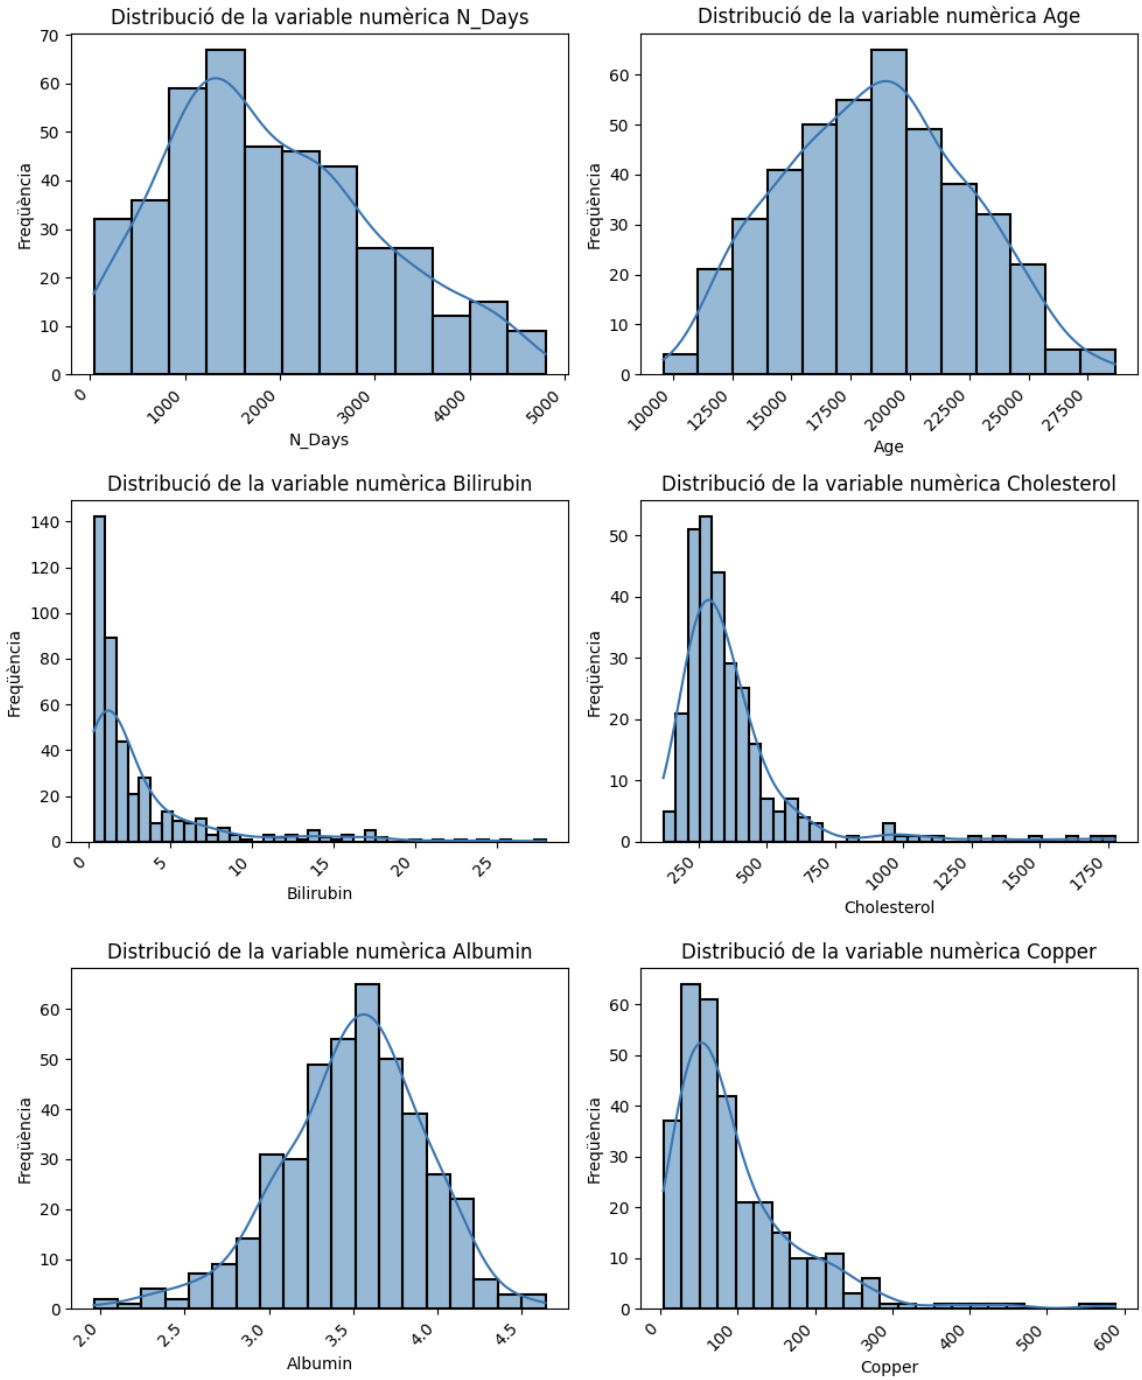
\includegraphics[width=\linewidth]{img/num-histograms-1.png}
    \caption{Histogrames de variables numèriques del datset.}
    \label{fig:num-histograms-1}
\end{figure}
\begin{figure}[H]
    \centering
    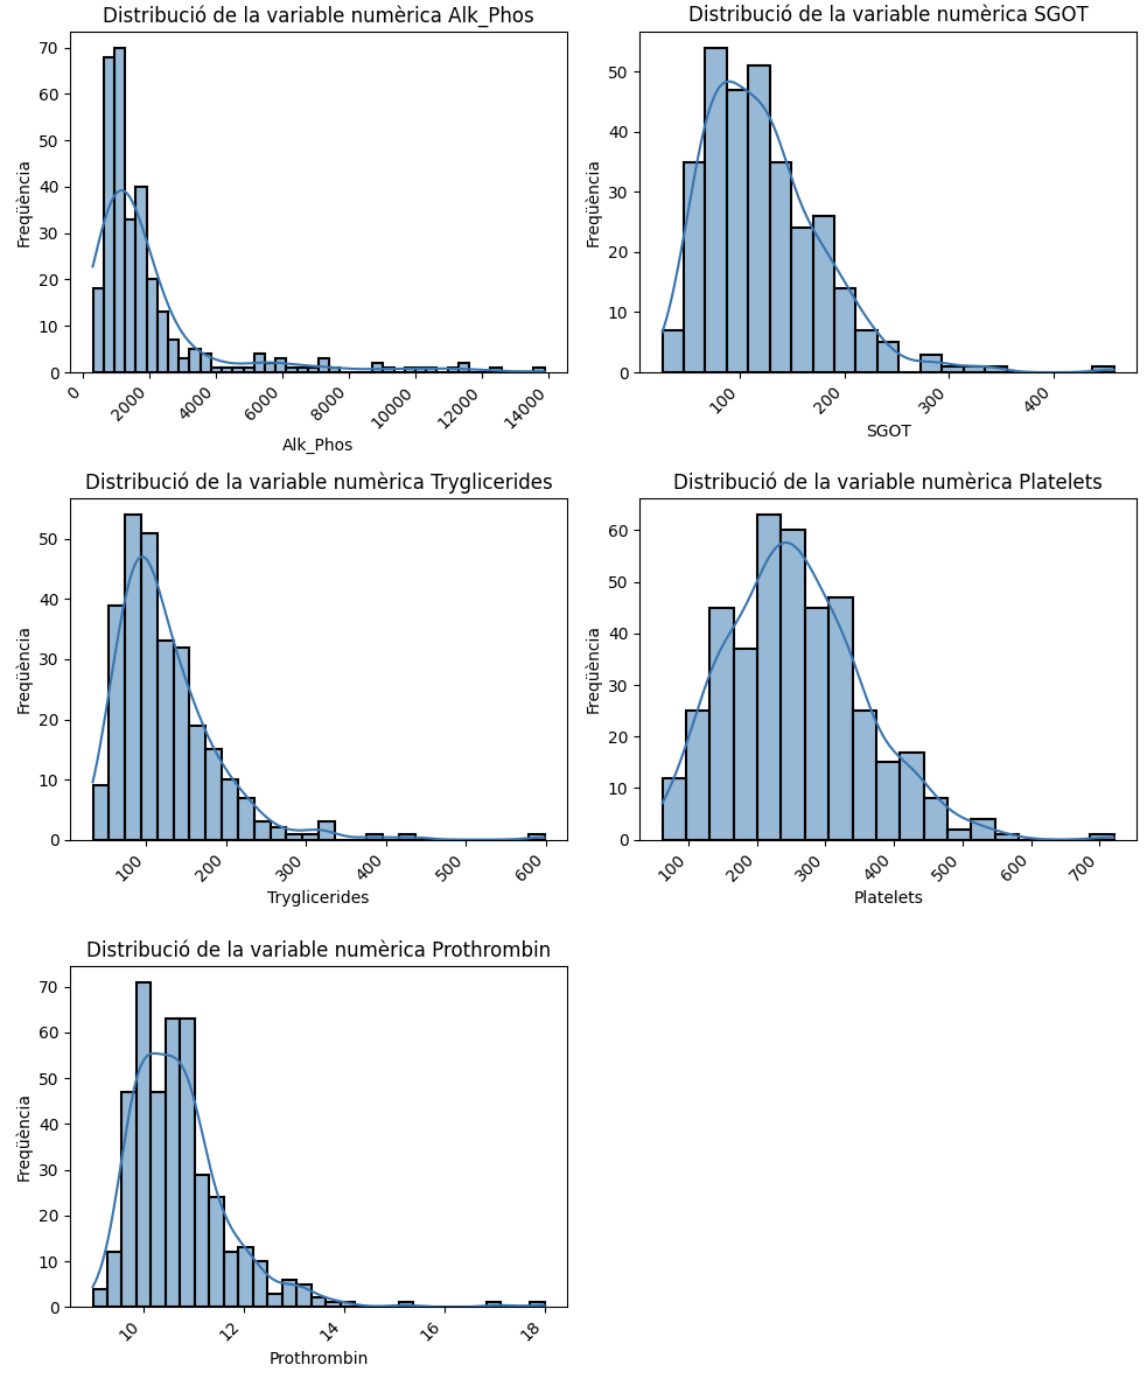
\includegraphics[width=\linewidth]{img/num-histograms-2.png}
    \caption{Histogrames de variables numèriques del datset.}
    \label{fig:num-histograms-2}
\end{figure}

En els histogrames de les diferents variables numèriques es pot veure com rarament segueixen una distribució normal. Això, en certs casos s'ha de tenir en compte en els models per tal de millorar el seu rendiment.

Per altra banda, també es pot veure que hi ha certes variables que tenen valors bastant allunyats de la distribució principal de les dades de la variable (valors atípics o outliers, que es tractaran més endavant).

\subsubsection{Variables categòriques}
En la taula \ref{tab:cat-stats-1} podem veure altres estadístiques per les variables categòriques del dataset (obtingudes mitjançant la mateixa comanda, però amb el paràmetre \texttt{include=`category'}).

\begin{table}[H]
\centering
\begin{tabular}{lrrrrrrrr}
\hline
\textbf{Statistic} & \textbf{Status} & \textbf{Drug} & \textbf{Sex} & \textbf{Ascites} & \textbf{Hepatomegaly} & \textbf{Spiders} & \textbf{Edema} & \textbf{Stage} \\ 
\hline
count & 418 & 312 & 418 & 312 & 312 & 312 & 418 & 412.0 \\ 
unique & 3 & 2 & 2 & 2 & 2 & 2 & 3 & 4.0 \\ 
top & Alive & 1 & F & 0 & 1 & 0 & NoEdema & 3.0 \\ 
freq & 232 & 158 & 374 & 288 & 160 & 222 & 354 & 155.0 \\ 
\hline
\end{tabular}
\caption{Categorical data summary of the study.}
\label{tab:cat-stats-1}
\end{table}

A més, en les figures \ref{fig:cat-countplots-1} i \ref{fig:cat-countplots-2} es poden veure els countplots de cada una de les variables categòriques, on es veu la quantitat de mostres que hi ha per cada classe de la variable, evitant els valors faltants (missings).

\begin{figure}[H]
    \centering
    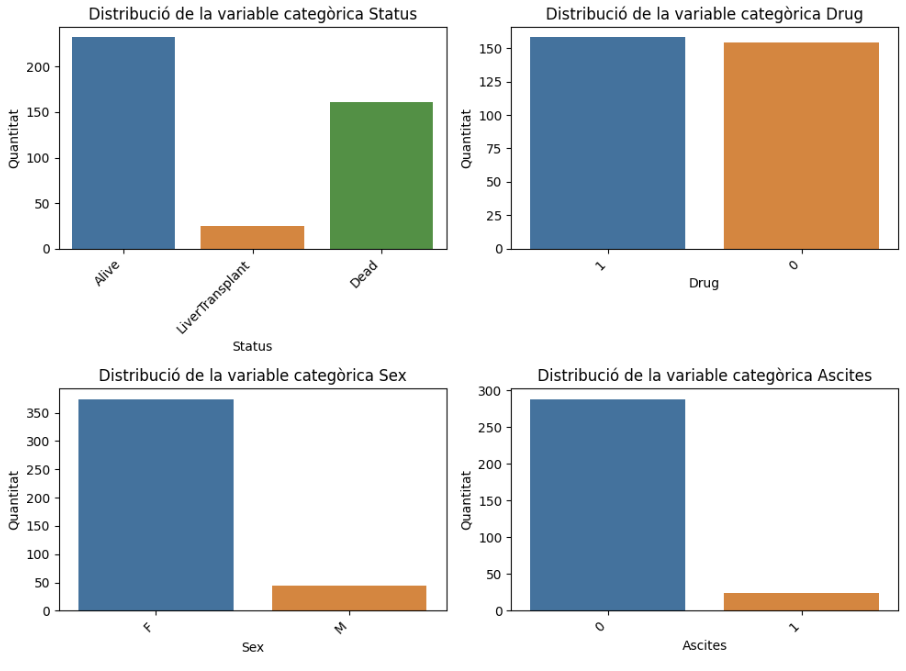
\includegraphics[width=\linewidth]{img/cat-countplots-1.png}
    \caption{Countplots de variables categòriques del datset.}
    \label{fig:cat-countplots-1}
\end{figure}
\begin{figure}[H]
    \centering
    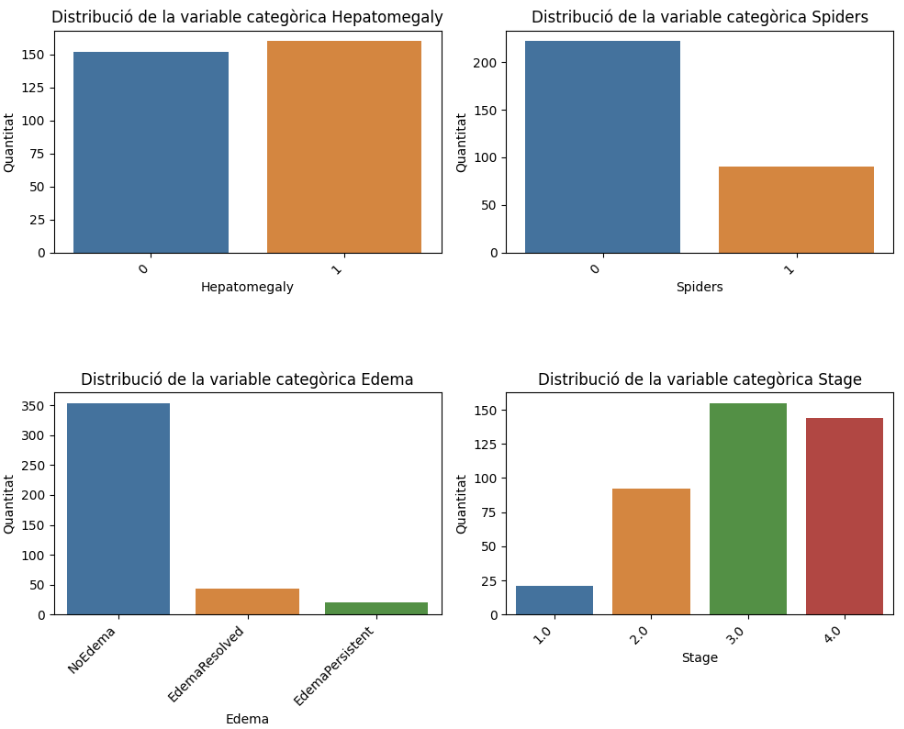
\includegraphics[width=\linewidth]{img/cat-countplots-2.png}
    \caption{Countplots de variables categòriques del datset.}
    \label{fig:cat-countplots-2}
\end{figure}

Es pot veure que les variables \textit{Status} (la variable que determinarem com a \textit{target} més endavant), \textit{Sex}, \textit{Ascites}, \textit{Spiders}, \textit{Edema} i \textit{Stage} pateixen un clar desbalanceig de classes. Per la variable \textit{Status} es contemplarà l'opció de realitzar un balanceig més endavant.

\subsection{Outliers}
El tractament d'outliers en models de Machine Learning pot ser molt important per millorar el seu rendiment mitjançant l'eliminació de mostres que es consideren atípiques. En la nostra base de dades, tal i com s'ha pogut veure en els histogrames de les variables numèriques (figures \ref{fig:num-histograms-1} i en les taules amb estadístiques de les variables (taules \ref{fig:num-histograms-2}) i en les taules \ref{tab:num-stats-1}, \ref{tab:num-stats-2} i \ref{tab:cat-stats-1}), hi ha unes quantes mostres que possiblement siguin outliers. Per exemple, la variable \textit{cholesterol} té un valor màxim de 1775, la qual cosa està exageradament per sobre de 240 (valor a partir del que es considera que una persona té un colesterol molt alt, segons la \textit{Fundación Española del Corazón} \cite{fundacioncorazon2023colesterol}).

Per eliminar aquests outliers, s'ha utilitzat l'Interquartile Range (IQR). Inicialment, un factor de multiplicació de 1,5 eliminava 119 files (un 28,47\% del dataset), resultant en menys de 300 files. Aquest valor semblava excessiu, així que s'ha optat per crear la funció \texttt{compare\_iqr\_factors()} per tal de visualitzar el percentatge de files eliminades per diversos factors multiplicatius del IQR (com es pot veure en la figura \ref{fig:iqr-factors}).

\begin{figure}[H]
	\centering
	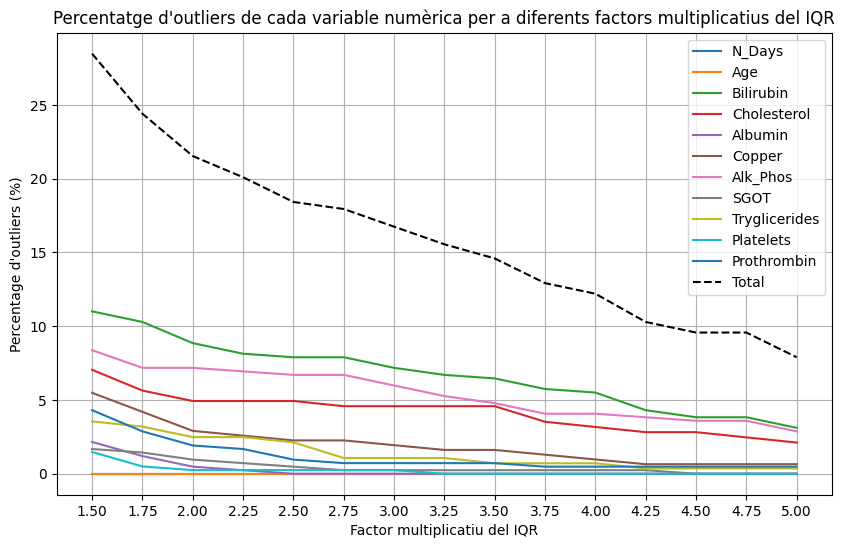
\includegraphics[width=0.85\linewidth]{img/iqr_factors}
    \caption{Percentatge de mostres considerades atípiques (outliers) en funció del factor multiplicatiu del IQR.}
    \label{fig:iqr-factors}
\end{figure}

Observant els resultats d'aquesta funció, s'ha decidit escollir un factor de 3, eliminant només 70 mostres (16,75\% del dataset). Aquesta selecció es justifica en les figures \ref{fig:outliers-1} i \ref{fig:outliers-2}, on es poden veure els histogrames i boxplots de les variables numèriques amb abans i després de l'eliminació d'outliers. En els historgrames, hi ha línia que indica a partir d'on es considera que una mostra és un outlier tenint en compte el factor de multiplicació 3. Fàcilment es pot apreciar que es consideren outliers només les mostres que se surten de la principal distribució de les dades de cada variable, reafirmant així la nostra selecció del factor de multiplicació del IQR és bona.

\begin{figure}[H]
\centering

\begin{subfigure}{.5\textwidth}
  \centering
  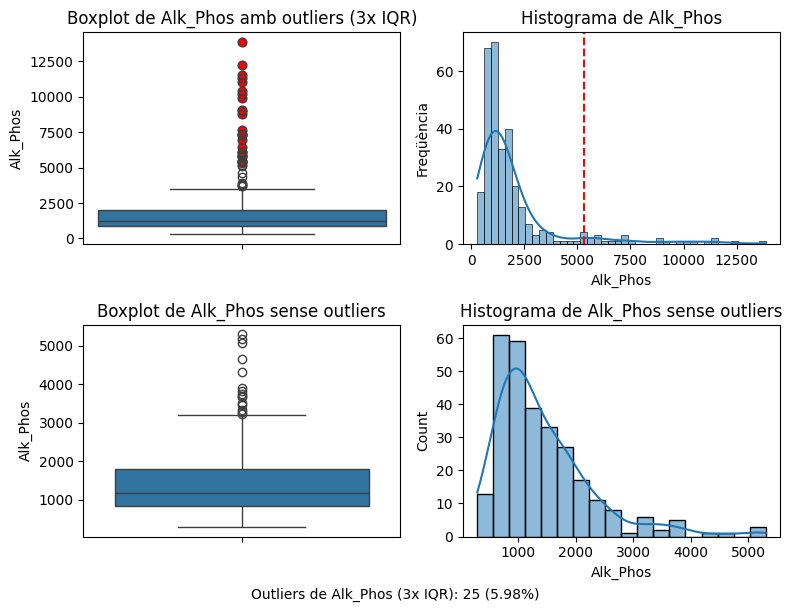
\includegraphics[width=.95\linewidth]{img/outliers_Alk_Phos.png}
  \caption{Alk\_phos}
\end{subfigure}%
\begin{subfigure}{.5\textwidth}
  \centering
  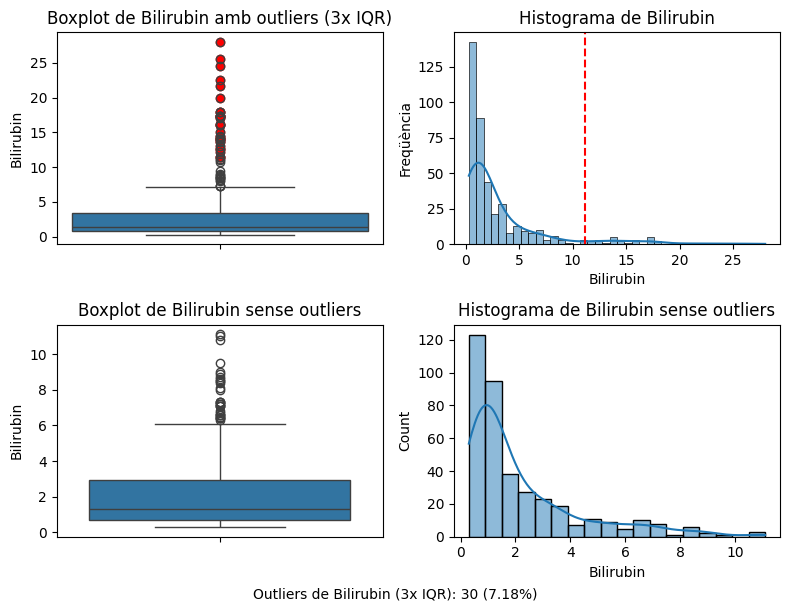
\includegraphics[width=.95\linewidth]{img/outliers_Bilirubin.png}
  \caption{Bilirubin}
\end{subfigure}
\begin{subfigure}{.5\textwidth}
  \centering
  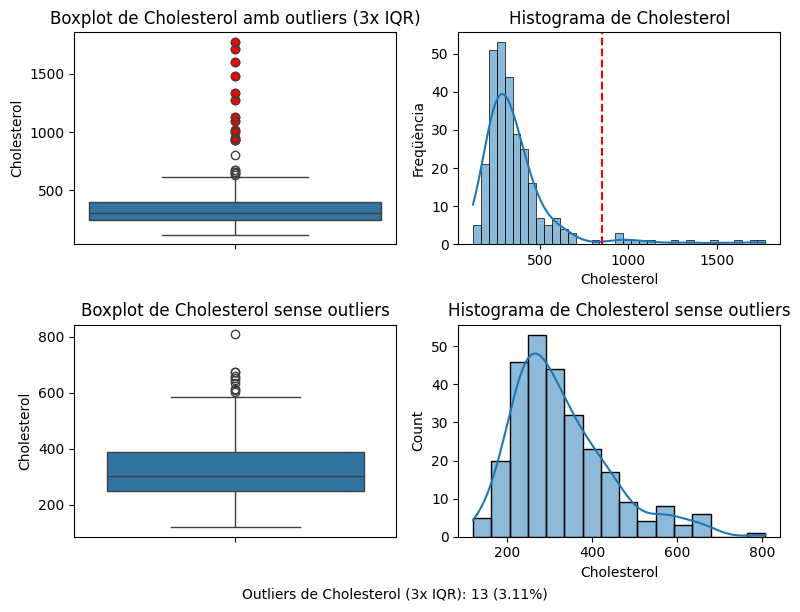
\includegraphics[width=.95\linewidth]{img/outliers_Cholesterol.png}
  \caption{Cholesterol}
\end{subfigure}%
\begin{subfigure}{.5\textwidth}
  \centering
  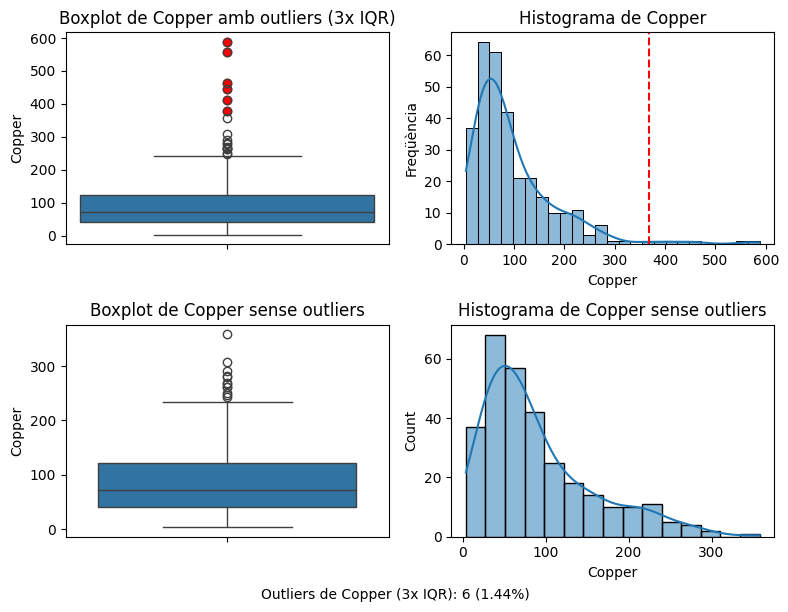
\includegraphics[width=.95\linewidth]{img/outliers_Copper.png}
  \caption{Copper}
\end{subfigure}

\caption{Distribució de dades de cada variable abans i després d'eliminar els outliers. La línia vermella discontínua dels histogramas indica a partir de on es consideren outliers les mostres. Els punts vermells dels boxplots representen outliers.}
\label{fig:outliers-1}
\end{figure}

\begin{figure}[H]
\centering

\begin{subfigure}{.5\textwidth}
  \centering
  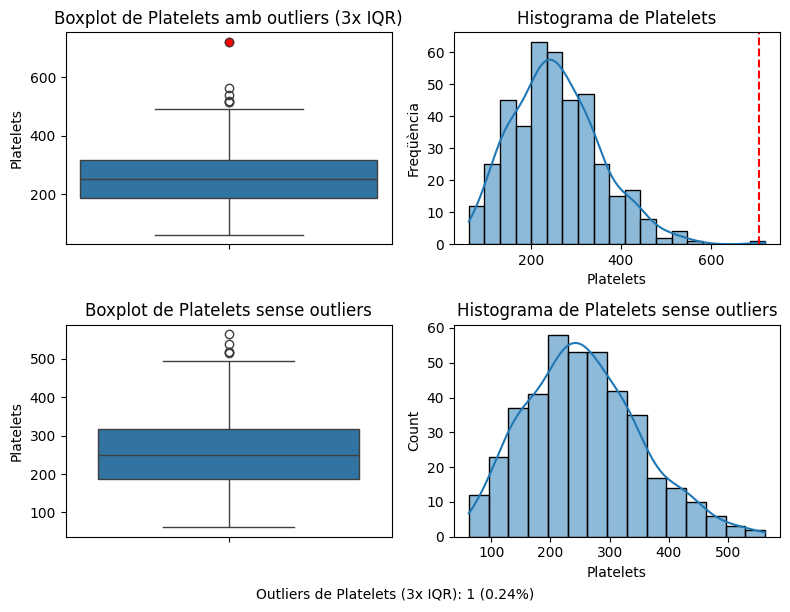
\includegraphics[width=.95\linewidth]{img/outliers_Platelets.png}
  \caption{Platelets}
\end{subfigure}%
\begin{subfigure}{.5\textwidth}
  \centering
  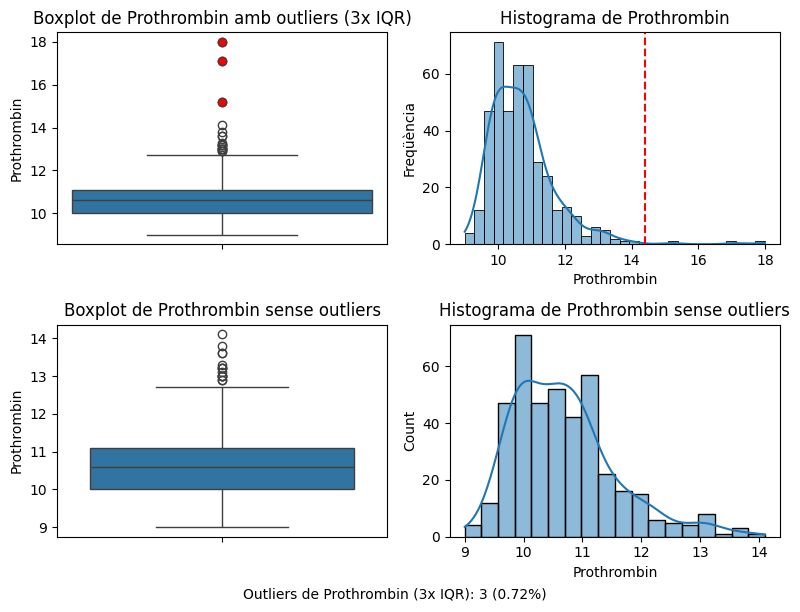
\includegraphics[width=.95\linewidth]{img/outliers_Prothrombin.png}
  \caption{Phtothrombin}
\end{subfigure}
\begin{subfigure}{.5\textwidth}
  \centering
  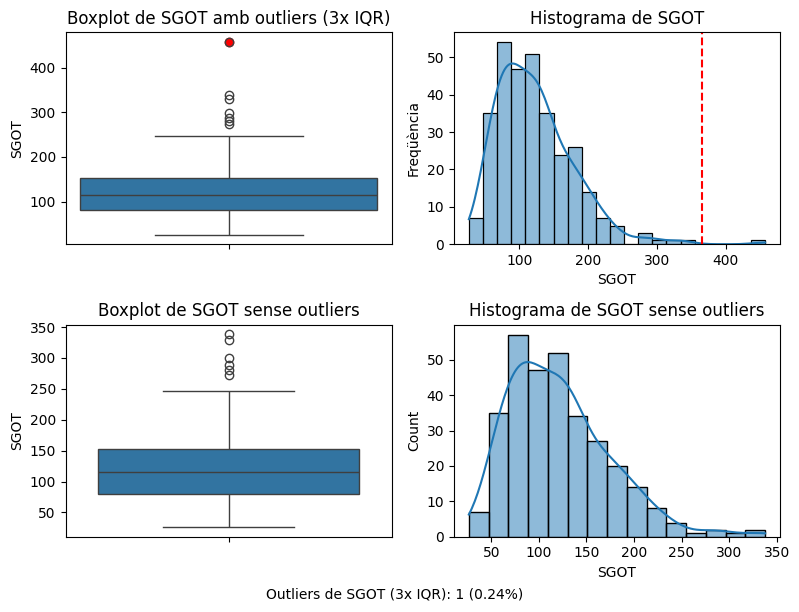
\includegraphics[width=.95\linewidth]{img/outliers_SGOT.png}
  \caption{SGOT}
\end{subfigure}%
\begin{subfigure}{.5\textwidth}
  \centering
  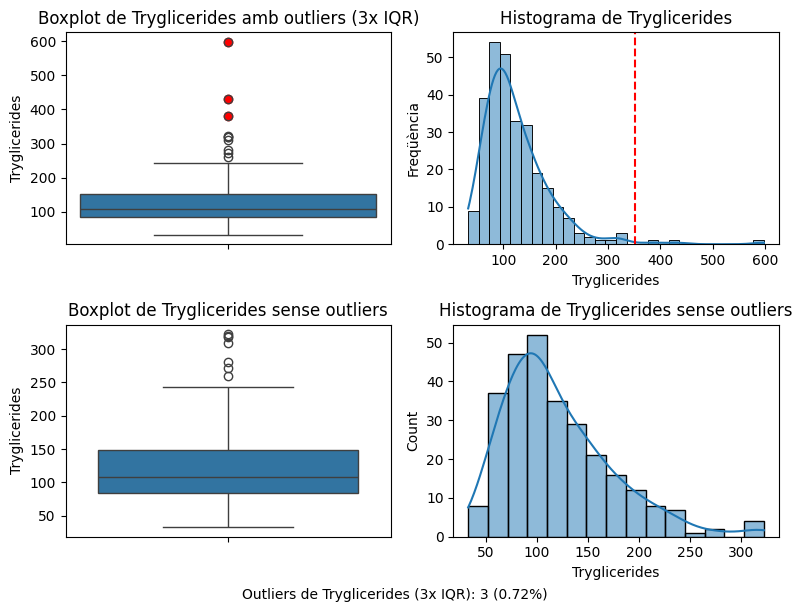
\includegraphics[width=.95\linewidth]{img/outliers_Tryglicerides.png}
  \caption{Tryglicerides}
\end{subfigure}

\caption{Distribució de dades de cada variable abans i després d'eliminar els outliers. La línia vermella discontínua dels histogramas indica a partir de on es consideren outliers les mostres. Els punts vermells dels boxplots representen outliers.}
\label{fig:outliers-2}
\end{figure}

Hem de considerar que no sempre s'obté un benefici en rendiment dels models quan s'eliminen outliers. A més, al tractar-se d'un datset amb dades de pacients malalts, podria ser que els valors que es detecten com a atípics siguin realment importants perquè el model aprengui els patrons de les dades per poder predir la nostra variable objectiu \textit{Status}. És a dir, segurament, totes les mostres del datset que contenen un nivell de colesterol extremadament alt tenen més probabilitat de morir, i eliminant outliers podem perdre part d'aquesta informació en certs casos. Per tant, l'eliminació d'outliers es valorarà per cada model més endavant, però sempre que es faci s'utilitzaran els criteris establerts en aquest estudi inicial de valors atípics (és a dir, s'utilitzarà el factor multiplicatiu del IQR de 3 mitjançant la funció \texttt{delete\_outliers}).

Per altra banda, cal mencionar que també existeix la possibilitat d'establir els valors atípics com a missings i imputar-los posteriorment. No obstant, com ja es mencionarà més endavant, ja hi ha una gran quantitat de valors faltants (missings) en el dataset, de manera que introduir-ne més només faria que hi hagués una proporció excessiva de valors imputats (que, evidentment, tenen una qualitat inferior als valors reals proporcionats en la pròpia base de dades).

\subsection{Particionat del dataset}
Per tal de poder entrenar i avaluar posteriorment els models, s'ha fet una partició del dataset en train i test. Degut a que disposem de poques mostres en la base de dades, s'ha optat per fer una partició de test de només el 15% de les dades. A més, en la partició de train es realitzarà cross validation en tots els models i també en la imputació de valors faltants per tal d'aprofitar millor la poca quantiat de mostres del datset i garantir un millor entrenament dels models.

Aquesta partició de la base de dades es fa en la funció \texttt{split\_dataset} i cal mencionar que la partició de test no s'utilitzarà en cap moment per entrenar models, ni per calcular mitjanes de cap variable del train, etc. És a dir, en tot moment es respectarà la independència de tots dos conjunts.

Finalment, cal mencionar també que, per tenir una proporció igual de classes de la variable objectiu (\textit{Status}) en tots dos conjunts, s'ha fet el perticionat mitjançant \textit{stratify} (conserva la distribució de classes en tots dos conjunts).

\subsection{Missings}
Inicialment el dataset conté una gran quantitat de missings. En la taula \ref{tab:missings} es pot veure que hi ha un total de 12 variables que contenen valors faltants. Observant el dataset inicial proporcionat, es pot veure que des de l'individu amb \textit{ID} = 313 fins al final del dataset (l'últim individu té \textit{ID} = 418) hi ha múltiples columnes que no tenen ni un únic valor (concretament, 9 columnes).

\begin{table}[H]
\centering
\begin{tabular}{lr}
\hline
\textbf{Variable} & \textbf{Nº de missings} \\
\hline
Tryglicerides & 136 \\
Cholesterol & 134 \\
Copper & 108 \\
Drug & 106 \\
Ascites & 106 \\
Hepatomegaly & 106 \\
Spiders & 106 \\
SGOT & 106 \\
Alk\_phos & 106 \\
Platelets & 11 \\
Stage & 6 \\
Prothrombin & 2 \\
\hline
\end{tabular}
\caption{Quantitat de valors faltants per cada variable amb almenys 1 missing.}
\label{tab:missings}
\end{table}

El dataset té molt poques mostres (418, com hem mencionat) i això pot portar problemes a l'hora de que el model aprengui (mitjançant l'entrenament). Sabent això, s'ha decidit que l'opció d'eliminar totes les files que continguin valors faltants no és viable, ja que es reduiria dràsticament la quantitat de mostres de la base de dades i no n'hi hauria suficients per tal de que els models trobessin bons patrons en la partició de train que farem més endavant. No obstant, per aquestes files concretes en què hi ha fins a 9 columnes amb valors faltants, s'ha implementat la funció \texttt{delete\_last\_rows()}, que les elimina del datset. Més endavant es faran proves per determinar si és útil eliminar aquestes files o és millor simplement imputar els valors.

Per imputar la resta de valors faltants s'han implementat les funcions \texttt{find\_best\_imputer()} i \texttt{impute\_data()}. La funció \texttt{impute\_data()} s'encarrega d'imputar els valors amb mètodes diferents (especificats en els paràmetres que introdueix l'usuari) per les variables numèriques i per les categòriques. Si es crida a la funció amb el paràmetre \texttt{numerical\_imputer = `best'}, es cridarà internament a la funció \texttt{find\_best\_imputer()} per trobar el millor imputador numèric. Per les variables categòriques succeeix el mateix, però amb el paràmetre \texttt{categorical\_imputer = `best'}.

Per altra banda, la funció \texttt{find\_best\_imputer()} implementa cross validation (sempre amb 5 particions/\textit{folds}) per trobar el millor imputador, tant numèric com categòric. El paràmetre \texttt{X\_train} és obligatori perquè, encara que s'estiguin intentant imputar els valors de la partició de test (que es menciona més endavant), s'escullen els millors mètodes d'imputació mitjançant només valors del train, per respectar totalment la independència entre les particions d'entrenament i de prova. El cross validation es fa sobre les mostres del train que no contenen missings i consisteix en generar artificialment valors faltants en cada \textit{fold} per posteriorment imputar-los i comprovar la seva eficàcia. Els mètodes d'imputació que es proven són els següents:
\begin{itemize}
	\item \textbf{Variables numèriques:}
		\begin{itemize}
		\item \textbf{KNNImputer:} aquest imputador es prova amb diferents valors de l'hiperparàmetre \textit{k} (1, 2, 3, 5, 10, 15, 20, 25, 50) i pot ser molt útil degut a que intenta imputar els valors basant-se en la mitjana dels valors dels deus \textit{k} veïns més propers.
		
		\item \textbf{SimpleImputer (mitjana):} aquest imputador és molt senzill. Simplement substitueix els valors faltants per la mitjana de la variable en què es trobi el valor missing. Generalment aquest mètode és pitjor que la resta, però s'ha volgut incloure igualment per si en algun cas proporciona un millor rendiment.
		
		\item \textbf{IterativeImputer (Linear Regression):} aquesta tècnica d'imputació és més complexa que les anteriors. L'iterative imputer pretén imputar els valors de cada variable mitjançant combinacions lineals de les altres. En aquest cas, es crea un model de regressió lineal per cada variable amb les altres variables com a predictores (sense tenir en compte els valors missing) i es fa una predicció per cada valor faltant. Al estar utilitzant una regressió lineal, el model rendirà millor si hi ha més relacions lineals entre variables numèriques del dataset.
		\end{itemize}

	\item \textbf{Variables categòriques:}
	Per les variables categòriques s'ha decidit utilitzar només classificadors, ja que altres mètodes no sempre funcionen per variables categòriques. S'ha de tenir en compte que en el moment d'imputar les dades encara no s'ha codificat el dataset (ja que codificar un dataset amb calors faltants és relativament complex i sovint genera errors). Per tant, les variables categòriques no poden ser utilitzades per algoritmes com ara KNN per tal de calcular les distàncies entre mostres. Per tant, predicció (imputació) de variables categòriques es fa, per cada variable categòrica, entrenant el classificador amb les variables numèriques.
	\begin{itemize}
		\item \textbf{KNeighborsClassifier:} aquest classificador obté resultats bastant diferents en funció de l'hiperparàmetre \textit{k}. Em aquest cas, es proven els mateixos valors de \textit{k} que en el KNNImputer utilitzat en les variables numèriques. Aquest classificador basa les seves prediccions en la moda (valor més freqüent) dels seus \textit{k} veïns més propers.
		\item \textbf{DecisionTreeClassifier:} en aquest cas s'imputen els valors mitjançant prediccions d'un arbre de decisió. Aquest arbre de decisió realitzarà, per cada variable categòrica, diverses particions del dataset en conjunts intentant mantenir homogeneïtat en cada un d'ells i posteriorment imputarà el valor faltant mitjançant la classe més freqüent en el conjunt on es situï la mostra a predir. En el nostre cas provem dos models, un amb el criteri d'entropia (entropy) i l'altre amb gini.
		
		\item \textbf{RandomForestClassifier:} aquest classificador es crea múltiples arbres de decisió i combina les seves prediccions. Generalment, el rendiment d'aquest classificador és més alt que el d'un sol arbre de decisió. En el nostre cas, també es prova tant amb el criteri entropy com amb gini.
	\end{itemize}
\end{itemize}

Tant els models de Decision Tree com els de Random Forest tenen bastants paràmetres que modifiquen el seu rendiment, especialment controlant si l'arbre fa més o menys overfitting. No obstant, s'ha decidit deixar els paràmetres per defecte per tal de no tenir una quantitat excessiva de models a provar en la funció \texttt{find\_best\_imputer()} i així reduir el cost computacional (i temps d'execució) d'aquesta funció. Més endavant, en el propi model de predicció de la variable objectiu mitjançant l'arbre de decisió, sí que es provaran diferents combinacions de paràmetres.

Pel que fa a l'elecció del millor model d'imputació, s'ha decidit que per les variables numèriques s'utilitzarà la mètrica de $R^2$ (coeficient de determinació). Un valor alt d'aquest coeficient significa que el model de imputació ha capturat un gran part de la variància dels valors reals, indicant que els valors predits s'assimilen als reals. S'ha escollit aquesta mètrica degut a que no depèn de l'escala de les dades, és robusta a outliers i és fàcilment interpretable.

Per altra banda, per avaluar l'imputador categòric s'ha decidit utilitzar la mètrica de \textit{f1}, ja que considera tant la precisió com el recall. A més, utilitzem la versió \textit{weighted} (ponderada) de la mètrica \textit{f1} per tal de tenir en compte el desbalanceig de les classes i per garantir que no s'obté una millor puntuació simplement pel fet d'estar predint (imputant) la classe majoritària de la variable.

En general, com es mencionarà més endavant, tots els models predictors de la variable target (\textit{Status}) també faran servir la mètrica de \textit{f1-score-weighted} pels mateixos motius.

Finalment, cal mencionar que la imputació de valors faltants sempre es farà per separat en les particions de train i test, per evitar data leakage i mantenir la independència dels dos conjunts.

\subsection{Recodificació de variables}
Com ja hem mencionat, en els models d'imputació de dades no s'han pogut tenir gaire en compte les variables categòriques degut a que no es poden fer operacions si no estan representades com a valors numèrics. Per altra banda, en el preprocessament inicial ja s'han passat certs valors de variables categòriques a format numèric per tal de poder treballar-hi més fàcilment. No obstant, ara que ja no hi ha valors faltants en el datset, pot ser molt útil realitzar una codificació de les variabels categòriques perquè els models de predicció de la variable objectiu (\textit{Status}) les puguin tenir en compte.

Hi ha múltiples mètodes de codificació de variables categòriques, com ara One Hot Encoding, Label Encoding, Ordinal Encoding, etc. Inicialment es va plantejar l'us de One Hot Encoding, però aquest codificador augmenta molt la dimensionalitat del dataset, redueix l'eficàcia dels càlculs, no manté la naturalesa dels valors de certes variables i dificulta molt la interpretació de la base de dades (crucial a l'hora de generar gràfics, comprovar que no hi hagi errors de valors en el dataset, etc.). Amb tot això, s'ha decidit descartar aquest encoder.

Pel que fa al Label Encoding i Ordinal Encoding, tots dos són bastant similars en el sentit de que simplement etiqueten cada una de les classes de les variables categòriques amb un número. No obstant, s'ha decidit utilitzar Ordinal Encoding, ja que hi ha variables que tenen un ordre natural en elles (com ara els valors de \textit{Stage}, que segueixen un ordre en funció de la fase en la que es trobi el pacient. És a dir, la fase 1 i la 3 estan ``més lluny'' que la 3 i la 4). Hi ha altres variables que no tenen un ordre en concret, però la majoria d'aquestes són binàries i no es veuran gaire afectades negativament pel fet de fer Ordinal Encoding. De fet, certs models com ara els arbres de decisió es poden veure beneficiats pel fet de tenir variables binàries (o que no tenen un ordre natural) expressades mitjançant Ordinal Encoding.

La codificació de variables es fa en la funció \texttt{encode\_variables}. Més endavant es faran proves per veure si és necessari fer encoding en tots els models o només en alguns.


\section{Preparació de variables}

\subsection{Normalització i escalat de variables}
En les variables numèriques, s'ha considerat l'ús de dues tècniques diferents per a l'escalat de dades: \textit{Standard Scaler} i \textit{MinMax Scaler}. El \textit{Standard Scaler} transforma les dades de manera que tinguin una mitjana de zero i una desviació estàndard d'una, mentre que el \textit{MinMax Scaler} redimensiona les dades en un rang entre 0 i 1.

Tenint en compte la nostra base de dades i l'ús que farem de les varianbles numèriques (princpalment per trobar distàncies entre mostres, etc.), s'ha decidit que, en general, el \textit{MinMax Scaler} és més útil o té més sentit per a la nostra aplicació. Aquesta decisió es basa en la manera en què el \textit{MinMax Scaler} preserva la relació entre les variables originals (mantenint les mateixes distàncies relatives), sent particularment beneficiós quan les característiques estan en diferents escales.

La normalització o l'escalat pot millorar significativament el rendiment dels nostres models (KNN, arbre de decisió i SVM), ja que es basen en les distàncies entre les punts o en la definició de marges entre les classes. Per tant, si s'ha de realitzar algun escalat es farà \textit{MinMax}. Arà bé, més endavant es valorarà per cada model si és millor realitzar ecalat o no.

Cal mencionar que escalat de dades es realitza sempre per separat en train i test, per tal de no tenir fuga de dades d'un conjunt a l'altre. A més, es fa abans d'imputar els valors faltants, ja que així els models d'imputació es poden beneficiar també dels avantatges de l'escalat de dades.

\subsection{Anàlisi de correlacions entre variables numèriques}
Per poder analitzar la correlació entre variables numèriques del dataset d'entrenament, s'ha fet una matriu de correlacions. No obstant, com ja s'ha mencionat, és possible que no s'utilitzi exactament la mateixa base de dades per entrenar tots els models. Per exemple, pot ser que en algun model es faci escalat de dades i en algun altre no, en algun s'eliminin outliers i en un altre no, etc..

Donada la gran quantitat de datasets d'entrenament que podem tenir en funció de les modificacions que hi fem, per realitzar la matriu de correlacions s'ha decidir fixar una llavor (\textit{seed}) per poder replicar els experiments i s'ha tingut en compte el dataset d'entrenament reultant a l'aplicar els següents canvis:
\begin{itemize}
	\item Llavor (random\_state) establerta arbitràriament al valor 42 en tots els processos que tinguin aleatorietat.
	\item Eliminació d'oultliers (amb factor multiplicatiu del IQR de 3).
	\item Sense eliminar les files amb 9 missings.
	\item Sense codificació de variables categòriques (això no hauria d'influir en les correlacions de variables numèriques, però s'especifica per si de cas).
	\item Escalat de variables numèriques mitjançant \textit{MinMax}.
	\item Missings imputats mitjançant els imputadors amb millors resultats amb la llavor escollida (mitjançant la funció \texttt{find\_best\_imputer()}) i determinats mitjançant la mètrica de $R^2$ (per variables numèriques) i \textit{f1-score-weighted} (per variables categòriques). Amb tot això, per a variables numèriques ha resultat ser millor l'IterativeImputer (amb Lineal Regression com a estimador), mentre que per a variables categòriques ha sigut el RandomForestClassifier amb el criteri gini.
	\item Sense realitzar cap mètode de balanceig de dades (explicats més endavant).
\end{itemize}

Tenint en compte totes aquestes consideracions, la matriu de correlacions entre variables numèriques resultant és la que es pot veure en la figura \ref{fig:num-corr}.

\begin{figure}[H]
	\centering
	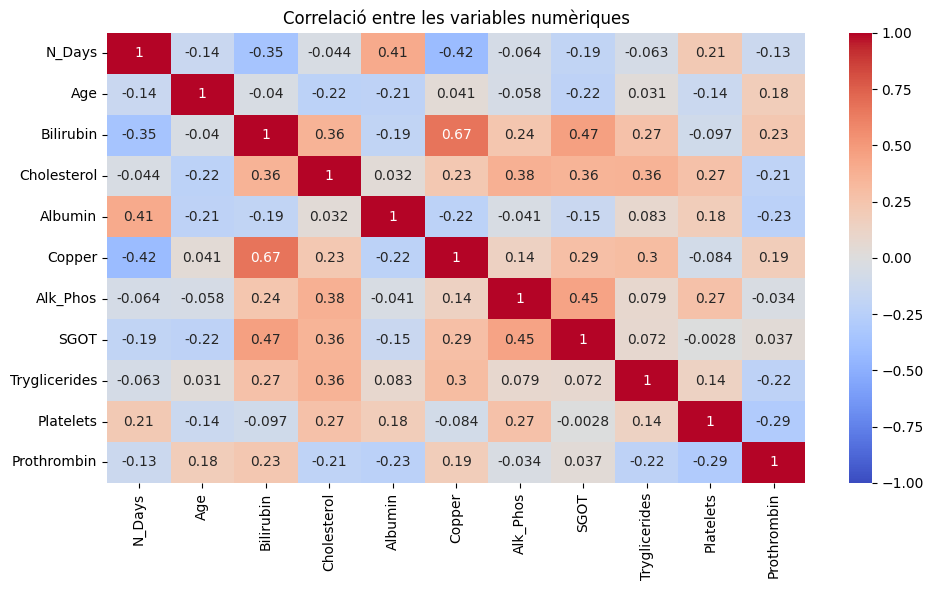
\includegraphics[width=0.9\linewidth]{img/num-corr.png}
	\caption{Matriu de correlacions entre totes les parelles de variables numèriques.}
	\label{fig:num-corr}
\end{figure}

Cal mencionar que la matriu de correlacions que es pot observar a la figura \ref{fig:num-corr} ens diu el coeficient de correlació per cada parella de variables, basant-se només en relacions lineals entre elles. Per tant, és possible que algunes de les variables numèriques tinguin clares relacions no lineals, però això no es pot apreciar en aquesta matriu.

La correlació entre \textit{Bilirubin} i \textit{Copper} és de 0,67, la qual cosa indica una forta correlació positiva. Això significa que a mesura que el valor de \textit{Bilirubin} augmenta, el valor de \textit{Copper} també tendeix a augmentar. 

\textit{Bilirubin} i \textit{SGOT} tenen una correlació positiva de 0,47, també bastant forta; i \textit{SGOT} i \textit{Alk\_Phos} de 0,45.

\textit{Copper} i \textit{N\_Days} destaquen pel que fa a les correlacions negatives, amb un coeficient de $-0,42$.

Finalment, la variable \textit{Cholesterol} té fins a 3 coeficients de correlació amb valors de 0,38, 0,36 i 0,36 amb les variables \textit{Alk\_Phos}, \textit{SGOT} i \textit{Tryglicerides}, respectivament.

Una vegada analitzades les correlacions més fortes, podem veure que les variables \textit{Bilirubin}, \textit{Copper}, \textit{SGOT} i \textit{Alk\_Phos} són les que es troben en més correlacions més fortes entre variables.

És important destacar que una correlació no implica causalitat. Això significa que, encara que dues variables estiguin correlacionades, no es pot assegurar que el valor d'una sigui causant del valor de l'altre. Per tant, no podem dir que el valor d'aquestes tres variables depengui dels altres, però en el nostre dataset d'entrenament es dona la casualitat (o potser causalitat) de que hi ha una alta correlació entre aquestes variables i altres variables del dataset.

Sabent tot això, si s'hagués d'eliminar alguna variable, les millors opcions per variables numèriques serien alguna de les 4 que hem mencionat, ja que part de la informació que aporten ja està explicada per altres variables. No obstant, s'ha considerat que, per la tasca de predicció de la variable objectiu i tenint en compte les dimensions del dataset, no cal eliminar cap variable numèrica per motiu de la seva correlació amb altres variables numèriques.

\subsection{Anàlisi de variables categòriques i variable objectiu}
Com que l'objectiu d'aquest projecte és acabar predint el valor de la variable \textit{Status}, és molt important veure com influeix el valor de la variable objectiu en cada variable categòrica.

Abans de res, cal mencionar que aquestes relacions han estat estudiades amb la mateixa base de dades d'entrenament que en l'apartat anterior. És a dir, aplicant exactament les mateixes modificacions al dataset inicial per tal de tenir el mateix conjunt de train. En funció del model que s'utilitzi posteriorment, aquest conjunt d'entrenament pot variar lleugerament.

En les figures \ref{fig:cat-target-1} i \ref{fig:cat-target-2} es poden veure aquestes relacions. Si entre els les diferents classes de la variable categòrica hi ha una distribució similar dels valors de la variable \textit{Status}, això ens indica que aquella variable categòrica no té gaire influència en la variable objectiu. Aquest és el cas de variables com \textit{Drug}.

Per altra banda, es pot veure que no hi ha cap variable amb una gran influència cap a la variable objectiu. A més, es destaca el desbalanceig de la variable objectiu, que tractarem a continuació. 

Amb tot el que s'ha vist, podem dir que si fos necessari eliminar una variable categòrica de l'entrenament, es podria eliminar la variable \textit{Drug}, ja que sembla ser la que menys influeix en la variable objectiu. No obstant, s'ha considerat que no és necessari eliminar-la degut a les característiques del nostre dataset.

És interessant observar que, si ens parem a pensar en la conclusió d'aquest anàlisi, s'ha mencionat que la variable \textit{Drug} (que originalment tenia valors `D-penicillamine' i `Placebo', i al preprocessing inicial s'han reemplaçat per 1 i 0, respectivament) no té pràcticament influència en la variable \textit{Status} (que indica si un pacient ha sobreviscut o no a la malaltia). Per tant, això ens està indicant que el tractament que es va utilitzar per realitzar aquest estudi sobre la cirrosis hepàtica no era efectiu. És a dir, els pacients que se'ls proporcionava el tractament (\textit{Drug} = `D-penicillamine', ara modificat a \textit{Drug} = 1) tenien les mateixes possibilitats de morir/sobreviure que els pacients que se'ls proporcionava un simple placebo.

\begin{figure}[H]
\centering
\begin{subfigure}[b]{0.5\textwidth}
    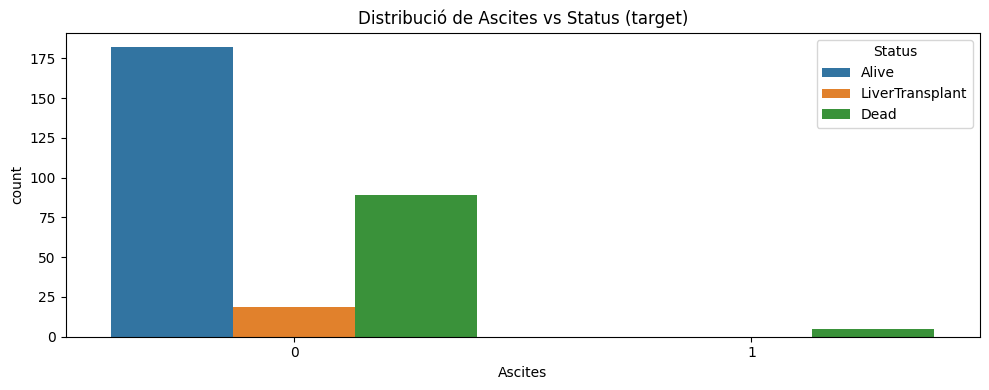
\includegraphics[width=\textwidth]{img/corr_Ascites_vs_status.png}
    \caption{Ascites vs status}
    \label{fig:ascites_vs_status}
\end{subfigure}%
\begin{subfigure}[b]{0.5\textwidth}
    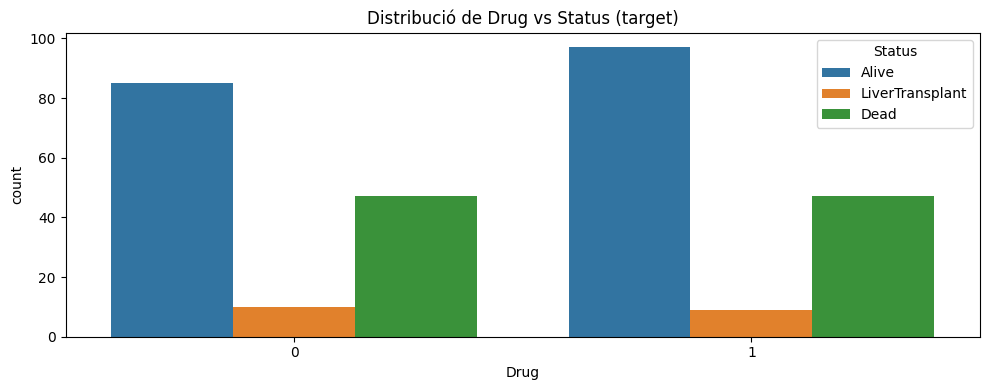
\includegraphics[width=\textwidth]{img/corr_Drug_vs_status.png}
    \caption{Drug vs status}
    \label{fig:drug_vs_status}
\end{subfigure}
\begin{subfigure}[b]{0.5\textwidth}
    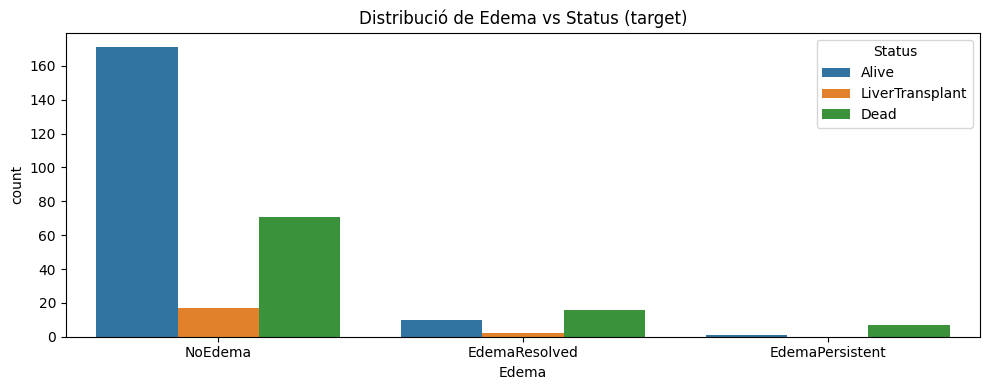
\includegraphics[width=\textwidth]{img/corr_Edema_vs_status.png}
    \caption{Edema vs status}
    \label{fig:edema_vs_status}
\end{subfigure}%
\begin{subfigure}[b]{0.5\textwidth}
    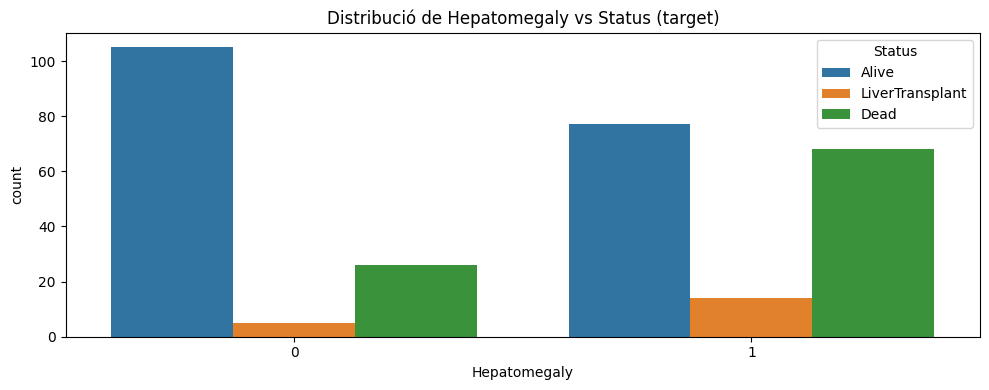
\includegraphics[width=\textwidth]{img/corr_Hepatomegaly_vs_status.png}
    \caption{Hepatomegaly vs status}
    \label{fig:hepatomegaly_vs_status}
\end{subfigure}
\caption{Relació entre les variables categòriques i la variable objectiu (\textit{Status})}
\label{fig:cat-target-1}
\end{figure}

\begin{figure}[H]
\centering
\begin{subfigure}[b]{0.5\textwidth}
    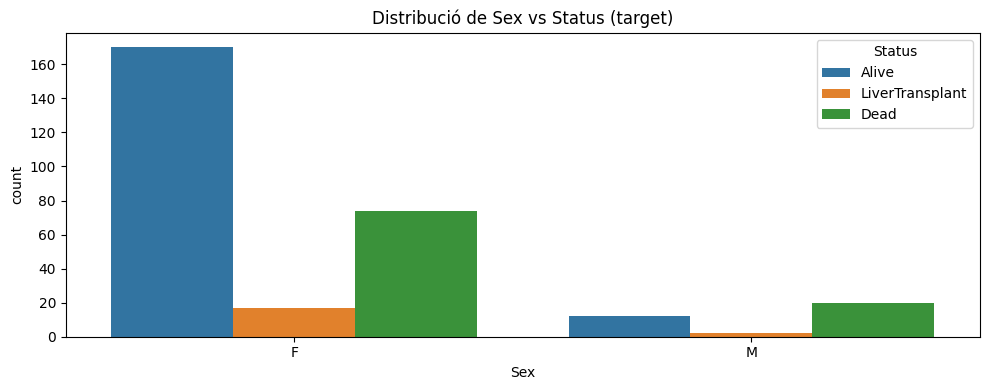
\includegraphics[width=\textwidth]{img/corr_Sex_vs_status.png}
    \caption{Sex vs status}
    \label{fig:sex_vs_status}
\end{subfigure}%
\begin{subfigure}[b]{0.5\textwidth}
    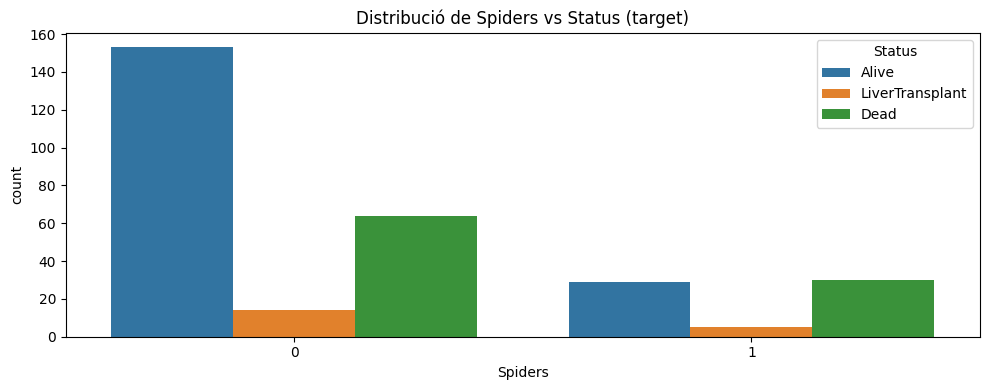
\includegraphics[width=\textwidth]{img/corr_Spiders_vs_status.png}
    \caption{Spiders vs status}
    \label{fig:spiders_vs_status}
\end{subfigure}
\begin{subfigure}[b]{0.5\textwidth}
    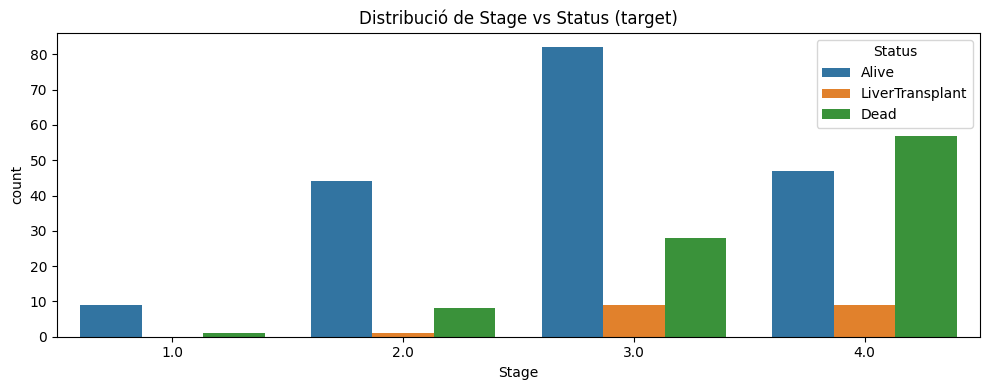
\includegraphics[width=\textwidth]{img/corr_Stage_vs_status.png}
    \caption{Stage vs status}
    \label{fig:stage_vs_status}
\end{subfigure}%
\begin{subfigure}[b]{0.5\textwidth}
    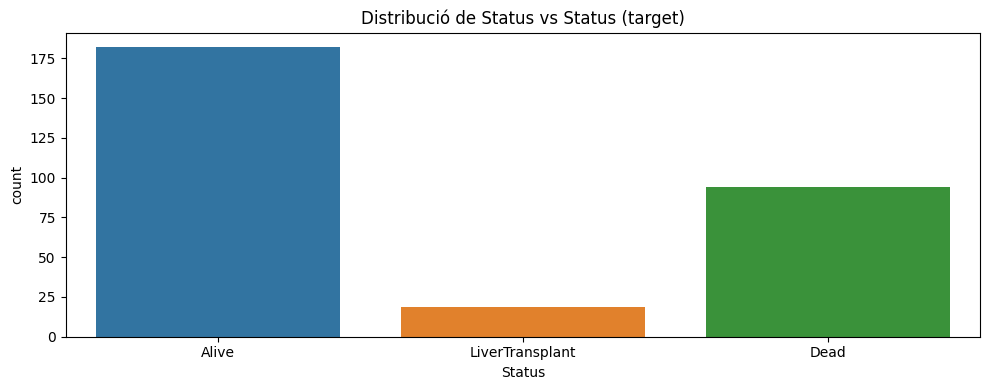
\includegraphics[width=\textwidth]{img/corr_Status_vs_status.png}
    \caption{Status vs status}
    \label{fig:status_vs_status}
\end{subfigure}
\caption{Relació entre les variables categòriques i la variable objectiu (\textit{Status})}
\label{fig:cat-target-2}
\end{figure}

\subsection{Balanceig de classes de la variable objectiu}
Com ja hem vist en la figura \ref{fig:status_vs_status}, la variable objectiu (\textit{Status}) està clarament desbalancejada. Hi ha moltes mostres amb valor `Alive', unes quantes amb valor `Dead' i molt poques amb valor `LiverTransplant'.

Això pot causar que els nostres models es dediquin a predir la classe majoritària i tinguin molt mal rendiment predient valors de la classe minoritària. Per poder solucionar-ho, s'han implementat diversos mètodes de balanceig de dades en la funció \texttt{balance\_target\_classes()} per aplicar al conjunt d'entrenament. En concret, s'ha implementat Oversampling, Undersampling, SMOTE i SMOTEENN.

Degut a la poca quantiat de dades del nostre dataset, ja podem saber que no té cap mena de sentit intentar aplicar Undersample, ja que ens quedaríem amb molt poques dades en el conjunt d'entrenament.

El mètode de Oversampling pot ser útil degut a la seva senzillesa. Simplement replica mostres del datset fins que les classes estan equilibrades. No obstant, s'ha d'anar amb compte amb aquest mètode perquè pot provocar overfitting.

El mètodes de SMOTE consisteix en generar mostres sintètiques basant-se en combinacions lineals dels veïns més propers. Aquest mètode és computacionalment més car, però redueix el risc de sobreajustament (overfitting) en comparació al Oversample.

Finalment, el mètode SMOTEENN es basa en un SMOTE, però posteriorment elimina aquelles mostres que considera de pitjor qualitat. Aconsegueix un menor balanceig de classes però assegura una millor qualitat de les mostres generades sintèticament.

Tots aquests mètodes es provaran més endavant per cada model i es determinarà quin és el que proporciona millors resultats per a cada un. Cal mencionar que tant SMOTE com SMOTEENN requereixen que les dades hagin estat codificades, ja que no poden tractar valors que no siguin numèrics. Així doncs, quan el dataset no ha estat codificat, no es podrà aplicar cap d'aquests dos mètodes.

\subsection{Eliminació de variables}
Pel que fa a la eliminació de possibles variables, ja s'ha mencionat en apartats anteriors que no s'ha considerat necessari en aquest projecte. El dataset té una mida relativament petita i no hi ha variables extremadament redundants o sorolloses. Per tant, eliminar variables no és necessari.

En cas que es volgués eliminar alguna variable numèrica, ja s'ha mencionat que les millors opcions serien \textit{Bilirubin}, \textit{Copper}, \textit{SGOT} o \textit{Alk\_Phos}. Per altra banda, en les variables categòriques s'optaria per eliminar \textit{Drug}.

\subsection{Estudi de dimensionalitat (ACP)}
En aquest apartat s'ha realitzat un estudi sobre la dimensionalitat de la base de dades d'entrenament mitjançant l'Anàlisi de Components Principals (ACP o PCA).

\begin{figure}[H]
    \includegraphics[width=0.85\textwidth]{img/acp.png}
    \caption{Status vs status}
    \label{fig:status_vs_status}
\end{figure}



\section{Definició de models}
Per la predicció de la variable objectiu (\textit{Status}) s'han realitzat 3 tipus diferents de models: un K-Nearest Neighbors (KNN), un Arbre de Decisió (Decision Tree) i un Support Vector Machine (SVM). 

En primer lloc, cal mencionar que tots aquests models treballen amb dades numèriques, de manera que requereixen que les dades categòriques hagin estat codificades. No obstant, en la implementació que s'ha fet, es contempla el cas en què les variables categòriques no han estat codificades i llavors el model prediu només amb les variables categòriques. Això ens permet poder fer proves amb i sense codificar les dades, ja que en certs models i datasets potser s'obté millor rendiment obviant les variables numèriques en la predicció.

Per cada un dels models, es definiran uns paràmetres generals fixes (els que generalment venen per defecte en els predictors de \texttt{scikit-learn}) i es provaran totes les possibles combinacions de modificacions al dataset (codificar o no, eliminar o no outliers, escalar variables o no, balancejar classes amb un mètode o amb un altre, etc.) mitjançant la funció \texttt{find\_best\_dataset()}. En cada una d'aquestes combinacions s'entrena el model i es fa la predicció, obtenint els resultats. El dataset (combinació de modificacions al dataset inicial) que aconsegueixi millors resultats (predient en el test) s'establirà com el ``millor dataset pels models d'aquell tipus''.

Una vegada determinat el millor dataset per cada tipus de model, es provaran moltes combinacions de paràmetres en les funcions \texttt{X\_prediction()} (on \texttt{X} serà \texttt{knn}, \texttt{dt} o \texttt{svm}, depenent del model) mitjançant cross validation en la partició de train. Els que donin millors resultats de mitjana en la validació s'utilitzaran per predir en el test i es determinarà com el ``model definitiu d'aquell tipus'' (ja que s'haurà entrenat amb un dataset específic per al model en concret i s'hauran trobat els paràmetres que rendeixen millor).

Evidentment, les proves es podrien fer directament sempre al test (no a la partició de validació) i també provar una major quantitat de paràmetres i combinacions de datasets dels que es provaran. No obstant, es considera que una de les parts fonamentals d'aquest projecte consisteix en saber filtrar què pot funcionar i què no, en comptes de provar-ho tot a la força bruta. És a dir, encara que els paràmetres que s'escullin en el validation no acabin sent els millors pel test (ja que poden estar donant mètriques més altes en el validation degut a overfitting), no és una solució eficient (ni en termes de computació, ni de temps, ni de escalabilitat, etc.) provar tots aquests paràmetres en el test directament. A més, les particions de validació estan fetes precisament per ajudar a escollir paràmetres.

Una vegada mencionat això, quan ja es tinguin els 3 ``models definitius'', es compararan els resultats per escollir el millor dels 3 models i procedir al seu anàlisi més exhaustiu, model card, etc.

Totes aquestes proves o execucions es realitzaran amb la llavor (seed o random\_state) amb valor 42 arbitràriament per una millor reproductibilitat. És evident que s'obtindrien millors resultats realitzant l'experiment amb múltiples llavors i escollint els paràmetres que més es repetissin en les diferents execucions (per així reduir el factor aleatori), però cada una d'aquestes execucions té una durada aproximada de 20 minuts, de manera que no és viable perdre-hi tant de temps. No obstant, si s'haguessin d'implementar aquests models en un cas real, seria molt important afegir més execucions amb llavors diferents per poder tenir resultats més robustos al factor aleatori.

A continuació es detallen els diferents tipus de models, els paràmetres provats, el conjunt de modificacions del dataset adient per cada un, les mètriques utilitzades, etc.

\subsection{K-Nearest Neighbors (KNN)}

\subsubsection{Motivació}
El nostre dataset conté dades relacionades amb pacients amb cirrosi hepàtica, on l'objectiu principal és predir l'estat del pacient (variable \textit{Status}). L'algorisme \textit{K-Nearest Neighbors} (KNN) es presenta com una elecció adequada per aquesta tasca per diverses raons.

En primer lloc, KNN és un algorisme basat en instàncies, el que significa que fa prediccions basant-se en la proximitat i similitud de les mostres en l'espai de característiques. Això és particularment útil en el nostre cas, on les característiques dels pacients com l'edat, sexe, indicadors bioquímics i la resposta al tractament poden influir directament en el seu estat de salut. La capacitat de KNN per capturar aquestes relacions espacials i fer prediccions sense la necessitat de que hi hagi patrons explícits el fa un bon candidat per conjunts de dades amb relacions complexes i no lineals entre les característiques i la variable objectiu.

A més, la naturalesa intuïtiva i la facilitat d'interpretació de KNN són avantatges significatius quan es tracta de dades mèdiques. La possibilitat de explicar les prediccions en termes de "pacients semblants" (\textit{Nearest Neighbors}) pot ser molt valuosa en l'àmbit mèdic, on la comprensió i la confiança en el model són també de gran importància.

\subsubsection{Mètriques}
Per l'avaluació del model, s'ha utilitzat la mètrica de \textit{f1-score-weighted}, tal i com s'ha dit que es faria en tots els models (inclosos els de imputació explicats en apartats anteriors). Aquesta mètrica és calcula fent la mitjana harmònica entre la \textit{precision} i el \textit{recall}, penalitzant els valors extrems (calen valors bons tant de \textit{precision} com de \textit{recall} per tal de tenir un bon \textit{f1}). La mitjana de valors de totes les prediccions es fa ponderada (\textit{weighted}), de manera que a cada classe se li dona una importància proporcional a les seves aparicions. D'aquesta manera, es puntua millor que s'aconsegueixi classificar correctament la classe majoritària (on s'haurà de fer més prediccions). 

Si en un altre experiment es desitgés predir donar molta importància la classe minoritària (en aquest cas ``LiverTransplant'', que no és tant rellevant en aquest estudi com ``Alive'' o ``Dead'') es podrien utilitzar altres mètriques que ho tinguessin més en consideració.

\subsubsection{Hiperparàmetres}
L'únic hiperparàmetre que s'ha modificat és la \textit{k} (\texttt{n\_neighbors} en la implementació de \texttt{scikit-learn}), que indica el nombre de veïns més propers que es consideren a l'hora de fer la predicció. Els valors que s'han provat són 1, 2, 3, 5, 10, 15, 20 ,25 i 50.

\subsubsection{Millor conjunt de dades}
Per trobar el conjunt de dades que proporciona un millor rendiment a aquest model, s'han fixat els hiperparàmetres a $k = 3$ i s'ha executat la funció \texttt{find\_best\_dataset()}. Després que es provin totes les combinacions possibles de modificacions al dataset inicial (un total de 64 combinacions), la que ha obtingut millors resultats de \textit{f1-score-weighted} en el test és la següent:
\begin{itemize}
	\item No eliminar outliers.
	\item Eliminar les files amb més de 9 NaNs.
	\item Escalar les variables numèriques amb \textit{MinMax}.
	\item Imputar variables numèriques amb KNN Imputer (amb $k = 15$) i les categòriques amb Random Forest Classifier (amb el criteri `gini'). Els resultats de la imputació (calculats tal i com s'ha explicat en l'apartat \ref{subsec:missings}) han estat de 0,3808 de mitjana entre la puntuació $R^2$ de les numèriques i \textit{f1-score-weighted} de les categòriques.
	\item No codificar les variables categòriques.
	\item No balancejar les classes de la variable objectiu.
\end{itemize}

Amb aquestes modificacions i els paràmetres fixes que s'han mencionat, s'ha aconseguit un resultat de 0,7838 de \textit{f1-score-weighted} en el conjunt de prova (test), que es pot considerar un resultat bastant bo. La partició de train conté 277 mostres i la de test 50. A partir d'aquí s'ha considerat que aquests són els millors conjunts de dades per els models KNN, i el següent pas serà trobar els millors paràmetres per el model en aquest dataset.

\subsubsection{Millors hiperparàmetres pel dataset escollit}
Una vegada determinat el millor dataset per els models KNN, cal provar quins són els millors paràmetres. Això es fa mitjançant la funció \texttt{run\_experiment()} que cridarà a \texttt{knn\_prediction()}. En aquesta segona funció s'implementa cross validation amb 5 \textit{folds} per cada possible combinació de paràmetres. Una vegada s'hagin provat tots els paràmetres, la combinació de paràmetres que tingui un millor \textit{f1-score-weighted} de mitjana en la partició de validació (és a dir, el que obtingui una millor puntuació en la validació creuada) es determinarà com la millor per el model KNN i s'executarà la predicció en el test.

Una vagada s'ha fet la l'execució, s'ha obtingut que el millor paràmetre és $k = 25$, amb una puntuació en la partició de validació de 0,6287.

\subsubsection{Resultats}
Amb el dataset escollit i els millors hiperparàmetres triats, la predicció en el conjunt ha obtingut les mètriques que es poden veure en la taula \ref{tab:knn-test}

\begin{table}[H]
\centering
\begin{tabular}{l|l}
\hline
\textbf{Metric} & \textbf{Value} \\
\hline
accuracy & 0.76 \\
f1-micro & 0.76 \\
f1-macro & 0.5228251507321274 \\
f1-weighted & 0.736537677002583 \\
precision-micro & 0.76 \\
precision-macro & 0.5075757575757576 \\
precision-weighted & 0.7145454545454545 \\
recall-micro & 0.76 \\
recall-macro & 0.539072039072039 \\
recall-weighted & 0.76 \\
\hline
\end{tabular}
\caption{Mètriques obtingudes en l'execució de KNN en la partició de test amb el millor dataset pel model i els millors paràmetres ($k = 25$).}
\label{tab:knn-test}
\end{table}

Si ens fixem en la mètrica que hem escollit (\textit{f1-score-weighted}), podem veure que s'ha obtingut un valor de 0,7365, que està bastant bé. Aquest valor és més alt del que s'ha obtingut en la partició de validació. Això segurament succeeix per un factor aleatori.

Pel que fa a les prediccions, en la figura \ref{fig:knn-cm} es pot veure la matriu de confusió d'aquest model en les prediccions del conjunt de test. Es pot apreciar que la majoria de prediccions són bones. No obstant, hi ha hagut 5 mostres `Alive' que s'han predit com a `Dead' i 4 mostres de `Dead' que s'han predit com `Alive', de manera que el model no és perfecte i en alguns casos s'equivoca. Pel que fa a la classe `LiverTransplant', hi ha molt poques mostres (només 3) i el model no ha sigut capaç de predir-les correctament, ja que les ha predit com a `Alive'. Tot i això, cal considerar que realment els pacients que ha tingut un transplant de fetge (`LiverTransplant') han acabat sobrevivint... de manera que aquest error en la predicció és menys greu que els de les altres classes.

Per poder extreure més conclusions sobre les prediccions de `LiverTransplant' seria útil conèixer en quines condicions una persona pot acabar rebent un transplant de fetge. És a dir, el pacient ha de complir unes condicions de salut per tal de que es faci el transplant o simplement cal que s'aconsegueixi un donador? Això podria ajudar a determinar millor si és millor que els valors que nos s'han predit correctament de `LiverTransplant' es prediguin com a `Alive' o com a `Dead'.

\begin{figure}[H]
	\centering
	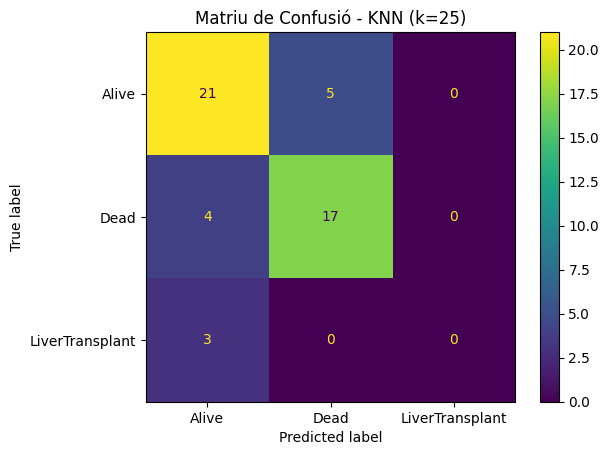
\includegraphics[width=0.85\linewidth]{img/knn-cm.png}
	\caption{Matriu de confusió de les prediccions del KNN (amb paràmetres $k = 25$) en el conjunt de test.}
	\label{fig:knn-cm}	
\end{figure}

Tot i el desbalanceig de classes, el model és aproximadament igual de bo predint la classe `Alive' (amb una proporció de $\dfrac{21}{26} \approx 0.8077$ prediccions correctes en aquesta classe) que la classe `Dead' (amb una proporció de $\dfrac{17}{21} \approx 0.8095$ prediccions correctes en aquesta classe).

%--------------------------------------------------------------------------
\subsection{Arbre de Decisió}

\subsubsection{Motivació}
El nostre dataset presenta dades complexes i diverses sobre pacients amb cirrosi hepàtica, on la tasca principal és predir l'estat del pacient (\textit{Status}). L'ús d'un arbre de decisió per a aquesta finalitat pot ser útil degut a que són models no lineals que poden capturar interaccions complexes entre les variables. Això és particularment útil en el nostre cas, ja que la condició dels pacients pot estar influenciada per una combinació de factors com ara l'edat, el sexe, els indicadors bioquímics, etc. . Un arbre de decisió pot dividir l'espai de les dades en subconjunts basats en aquestes característiques, facilitant la comprensió de com aquests factors interactuen i afecten el \textit{Status} del pacient.

\subsubsection{Mètriques}
De la mateixa manera que s'ha fet per al KNN, en l'avaluació del model s'ha utilitzat la mètrica de \textit{f1-score-weighted}. Aquesta mètrica és calcula fent la mitjana harmònica entre la \textit{precision} i el \textit{recall}, penalitzant els valors extrems (calen valors bons tant de \textit{precision} com de \textit{recall} per tal de tenir un bon \textit{f1}). La mitjana de valors de totes les prediccions es fa ponderada (\textit{weighted}), de manera que a cada classe se li dona una importància proporcional a les seves aparicions. D'aquesta manera, es puntua millor que s'aconsegueixi classificar correctament la classe majoritària (on s'haurà de fer més prediccions). 

Si en un altre experiment es desitgés predir donar molta importància la classe minoritària (en aquest cas ``LiverTransplant'', que no és tant rellevant en aquest estudi com ``Alive'' o ``Dead'') es podrien utilitzar altres mètriques que ho tinguessin més en consideració.

\subsubsection{Hiperparàmetres}
Pel que fa als hiperparàmetres de l'arbre de decisió, s'han modificat el criteri de decisió, la profunditat màxima, el nombre mínim de mostres per cada fulla i el nombre mínim de mostres per dividir un conjunt de l'arbre.

Els valors que es provaran per cada un dels paràmetres són els següents:
\begin{itemize}
	\item \textbf{Criteri}: `entropy' i `gini'.
	\item \textbf{Max\_depth}: None, 2, 3, 5, 10, 20, 50.
	\item \textbf{Min\_samples\_leaf}: 1, 2, 3, 5, 10, 20 ,50.
	\item \textbf{Min\_samples\_split}: 2, 3, 5, 10, 20, 50.
\end{itemize}

Totes les possibles combinacions d'aquests paràmetres es provaran mitjançant  Grid Search i cross validation per trobar els que millor rendiment aporten al model.

\subsubsection{Millor conjunt de dades}
Per trobar el conjunt de dades que proporciona un millor rendiment a aquest model, s'han fixat els següents hiperparàmetres:
\begin{itemize}
	\item \textbf{Criteri}: `entropy'.
	\item \textbf{Max\_depth}: None.
	\item \textbf{Min\_samples\_leaf}: 1.
	\item \textbf{Min\_samples\_split}: 2.
\end{itemize}

Amb aquests paràmetres fixats, s'ha executat la funció \texttt{find\_best\_dataset()}. Després que es provin totes les combinacions possibles de modificacions al dataset inicial (un total de 64 combinacions), la que ha obtingut millors resultats de \textit{f1-score-weighted} en el test és la següent:
\begin{itemize}
	\item No eliminar outliers.
	\item Eliminar les files amb més de 9 NaNs.
	\item No escalar les variables numèriques.
	\item Imputar variables numèriques amb Iterative Imputer (amb Lineal Regression com a estimador) i les categòriques amb Random Forest Classifier (amb el criteri `gini'). Els resultats de la imputació (calculats tal i com s'ha explicat en l'apartat \ref{subsec:missings}) han estat de 0,3581 de mitjana entre la puntuació $R^2$ de les numèriques i \textit{f1-score-weighted} de les categòriques.
	\item Codificar les variables categòriques amb \textit{Ordinal Encoding}.
	\item Balancejar les classes de la variabe objectiu mitjançant \textit{Oversampling}.
\end{itemize}

Amb aquestes modificacions i els paràmetres fixes que s'han mencionat, s'ha aconseguit un resultat de 0,7849 de \textit{f1-score-weighted} en el conjunt de prova, que es pot considerar un resultat bastant bo. La partició de train conté 441 mostres i la de test 50. A partir d'aquí s'ha considerat que aquests són els millors conjunts de dades per els models d'Arbre de Decisió, i el següent pas serà trobar els millors paràmetres per el model en aquest dataset.

\subsubsection{Millors hiperparàmetres pel dataset escollit}
Una vegada determinat el millor dataset per els models d'Arbre de Decisió, cal provar quins són els millors paràmetres. Això es fa mitjançant la funció \texttt{run\_experiment()} que cridarà a \texttt{dt\_prediction()}. En aquesta segona funció s'implementa cross validation amb 5 \textit{folds} per cada possible combinació de paràmetres. Una vegada s'hagin provat tots els paràmetres, la combinació de paràmetres que tingui un millor \textit{f1-score-weighted} de mitjana en la partició de validació (és a dir, el que obtingui una millor puntuació en la validació creuada) es determinarà com la millor per el model d'Arbre de Decisió i s'executarà la predicció en el test.

Una vagada s'ha fet la l'execució, s'ha obtingut que la millor combinació de paràmetres és la següent:
\begin{itemize}
	\item \textbf{Criteri}: `gini'.
	\item \textbf{Max\_depth}: None.
	\item \textbf{Min\_samples\_leaf}: 1.
	\item \textbf{Min\_samples\_split}: 2.
\end{itemize}

Amb aquests paràmetres s'ha obtingut una puntuació en la partició de validació de 0,8319.

\subsubsection{Resultats}
Amb el dataset escollit i els millors hiperparàmetres triats, la predicció en el conjunt ha obtingut les mètriques que es poden veure en la taula \ref{tab:dt-test}

\begin{table}[H]
\centering
\begin{tabular}{l|l}
\hline
\textbf{Metric} & \textbf{Value} \\
\hline
accuracy & 0.7 \\
f1-micro & 0.7 \\
f1-macro & 0.5724135182528296 \\
f1-weighted & 0.7096724055475849 \\
precision-micro & 0.7 \\
precision-macro & 0.5666666666666667 \\
precision-weighted & 0.722 \\
recall-micro & 0.7 \\
recall-macro & 0.5897435897435898 \\
recall-weighted & 0.7 \\
\hline
\end{tabular}
\caption{Mètriques de les prediccions de l'Arbre de Decisió (amb paràmetres \textit{criterion = `gini', max\_depth = None, min\_samples\_leaf = 1} i \textit{min\_samples\_split = 2}) en el conjunt de test.}
\label{tab:dt-test}
\end{table}

Si ens fixem en la mètrica que hem escollit (\textit{f1-score-weighted}), podem veure que s'ha obtingut un valor de 0,7097, que és un valor considerablement bo. A més, en aquest cas el valor sí que es menor a l'obtingut en la validació creuada, de manera que podem dir que segurament el nostre model té un lleuger overfitting en les dades del train. Tot i això, a l'hora de generalitzar els resultats en el test, el nostre model és capaç de rendir suficientment bé.

Pel que fa a les prediccions, en la figura \ref{fig:dt-cm} es pot veure la matriu de confusió d'aquest model en les prediccions del conjunt de test. Es pot veure que la majoria de prediccions són bones, però hi ha hagut 6 mostres `Alive' que no s'han predit correctament, 7 de `Dead' i 2 de `LiverTransplant'. Per les classes, `Alive' i `Dead', el model és lleugerament pitjor que el KNN (i per això ha obtingut un \textit{f1-score-weighted} menor), però per `LiverTransplant' ha aconseguir fer almenys una predicció correcta.

\begin{figure}[H]
	\centering
	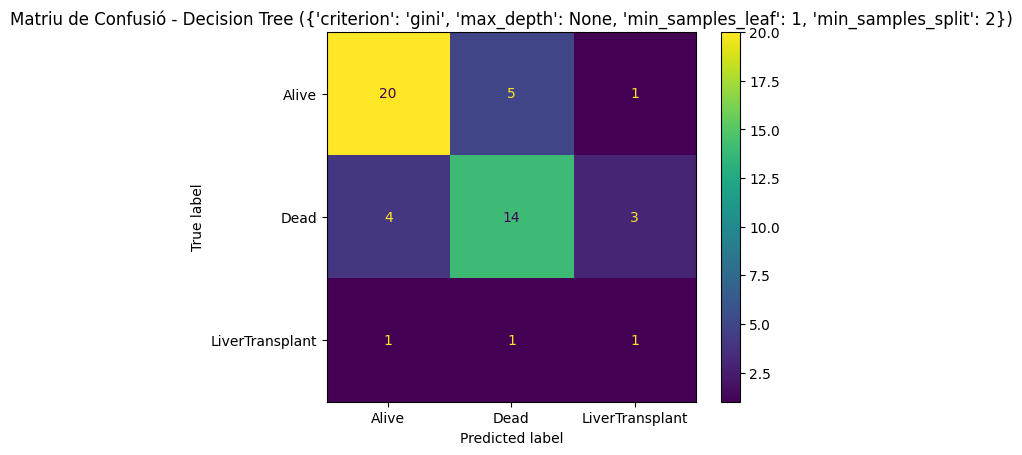
\includegraphics[width=0.95\linewidth]{img/dt-cm.png}
	\caption{Matriu de confusió de les prediccions de l'Arbre de Decisió (amb paràmetres \textit{criterion = `gini', max\_depth = None, min\_samples\_leaf = 1} i \textit{min\_samples\_split = 2}) en el conjunt de test.}
	\label{fig:dt-cm}	
\end{figure}

En aquest model, la classe `Alive' s'ha predit correctament en una proporció de $\dfrac{20}{26} \approx 0,7692$ i en la classe `Dead' $\dfrac{14}{21} \approx 0,6667$. Aquests resultats són pitjors que pel KNN i en aquest cas el model és millor predint la classe majoritària (`Alive'). Com ja hem dit, la part positiva d'aquest model és que ha aconseguir predir correctament una de les tres mostres de `LiverTransplant'; però, com que hi ha molt poques mostres, s'ha de tenir menys en compte aquesta classe.

%--------------------------------------------------------------------------
\subsection{Support Vector Machine (SVM)}

\subsubsection{Motivació}
Les SVM ofereixen una gran flexibilitat mitjançant l'ús de diferents funcions de kernel. Això ens permet explorar diferents maneres de modelar les relacions no lineals entre les variables i la variable objectiu "Status". Per exemple, un kernel polinòmic o de base radial (RBF) pot capturar relacions complexes que podrien ser crucials per la nostra predicció.

Un altre avantatge important de les SVM és la seva capacitat de controlar l'equilibri entre l'error de classificació i la complexitat del model a través del paràmetre de regularització C. Això és especialment útil quan es treballa amb dades mèdiques, on el balanç entre sensibilitat i especificitat és fonamental.

Finalment, la robustesa de les SVM davant dades amb soroll o outliers les fa una opció atractiva per a datasets complexos i desordenats com pot ser el nostre.

\subsubsection{Mètriques}
De la mateixa manera que s'ha fet per al KNN i per a l'Arbre de Decisió, en l'avaluació del model s'ha utilitzat la mètrica de \textit{f1-score-weighted}. Aquesta mètrica és calcula fent la mitjana harmònica entre la \textit{precision} i el \textit{recall}, penalitzant els valors extrems (calen valors bons tant de \textit{precision} com de \textit{recall} per tal de tenir un bon \textit{f1}). La mitjana de valors de totes les prediccions es fa ponderada (\textit{weighted}), de manera que a cada classe se li dona una importància proporcional a les seves aparicions. D'aquesta manera, es puntua millor que s'aconsegueixi classificar correctament la classe majoritària (on s'haurà de fer més prediccions). 

Si en un altre experiment es desitgés predir donar molta importància la classe minoritària (en aquest cas ``LiverTransplant'', que no és tant rellevant en aquest estudi com ``Alive'' o ``Dead'') es podrien utilitzar altres mètriques que ho tinguessin més en consideració.

\subsubsection{Hiperparàmetres}
Pel que fa als hiperparàmetres de la SVM, s'han modificat el kernel, el paràmetre C i el paràmetre gamma.

Els valors que es provaran per cada un dels paràmetres són els següents:
\begin{itemize}
	\item \textbf{Kernel}: `linear', `poly', `sigmoid', `rbf'.
	\item \textbf{C}: 0.1, 0.5, 1, 2, 3, 5.
	\item \textbf{Gamma}: `scale', `auto'.
\end{itemize}

El significat de cada paràmetre és el següent:
\begin{itemize}
	\item \textbf{Kernel}: aquest paràmetre representa la funció matemàtica que s'utilitzarà per transformar les dades a un espai de major dimensionalitat i així poder trobar relacions no lineals per separar les dades per un hiperplà. 
	\begin{itemize}
		\item `linear': aquest kernel no fa cap transformació, sinó que manté les dades en el seu espai original. És simple i computacionalment més barat.
		\item `poly': aquest kernel transforma les dades a un espai de major dimensió on les combinacions polinòmiques dels atributs originals esdevenen les noves dimensions. Permet modelar interaccions més complexes entre variables que el kernel lineal. El seu comportament depèn d'un paràmetre `degree' que controla el grau polinòmic. En el nostre cas, s'ha deixat sempre el grau per defecte, que és 3.
		\item `sigmoid': aquest kernel utilitza una funció sigmoide (semblant a la funció d'activació en xarxes neuronals). És capaç de transformar l'espai de dades de maneres no lineals i no polinòmiques.
		\item `rbf': aquest és un dels kernels més populars en les SVM. Transforma les dades a un espai on la distància radial (basada en la distància euclidiana) des d'un punt central determina el valor de cada nova dimensió. És molt efectiu per capturar relacions complexes en les dades i depèn del paràmetre gamma, que controla l'amplitud de la `zona d'influència' de cada un dels punts de suport.
	\end{itemize}	
	
	\item \textbf{C}: aquest paràmetre controla l'equilibri entre la maximització del marge i la minimització de l'error en la classificació. Un valor més alt penalitza més els errors i disminueix el marge (pot portar a overfitting); mentre que un valor més baix permet més errors i augmenta el marge (pot portar a underfitting).
	
	\item \textbf{Gamma}: aquest paràmetre és per el kernel `rbf' i controla si es té en compte una àrea més o menys gran per cada punt de suport a l'hora de determinar el límit de decisió.
	\begin{itemize}
		\item `scale': amb aquest paràmetre, la gamma s'adapta automàticament a l'escala de les dades. Ajuda a prevenir que el model sigui massa sensible a les variacions el les dades quan hi ha moltes dimensions o quan les característiques tenen variàncies molt diferents.
		\item `auto': aquest enfoc no té en compte la variància de les dades i pot no ser tant òptim som `scale' en certs casos.
	\end{itemize}		
\end{itemize}

Totes les possibles combinacions d'aquests paràmetres es provaran mitjançant  Grid Search i cross validation per trobar els que millor rendiment aporten al model.

\subsubsection{Millor conjunt de dades}
Per trobar el conjunt de dades que proporciona un millor rendiment a aquest model, s'han fixat els següents hiperparàmetres:
\begin{itemize}
	\item \textbf{Kernel}: `rbf'.
	\item \textbf{C}: 1.
	\item \textbf{Gamma}: 'scale'.
\end{itemize}

Amb aquests paràmetres fixats, s'ha executat la funció \texttt{find\_best\_dataset()}. Després que es provin totes les combinacions possibles de modificacions al dataset inicial (un total de 64 combinacions), la que ha obtingut millors resultats de \textit{f1-score-weighted} en el test és la següent:
\begin{itemize}
	\item No eliminar outliers.
	\item Eliminar les files amb més de 9 NaNs.
	\item Escalar les variables numèriques amb \textit{MinMax}.
	\item Imputar variables numèriques amb KNN Imputer (amb $k = 15$) i les categòriques amb Random Forest Classifier (amb el criteri `gini'). Els resultats de la imputació (calculats tal i com s'ha explicat en l'apartat \ref{subsec:missings}) han estat de 0,3808 de mitjana entre la puntuació $R^2$ de les numèriques i \textit{f1-score-weighted} de les categòriques.
	\item Codificar les variables categòriques amb \textit{Ordinal Encoding}.
	\item Balancejar les classes de la variabe objectiu mitjançant \textit{SMOTE}.
\end{itemize}

Amb aquestes modificacions i els paràmetres fixes que s'han mencionat, s'ha aconseguit un resultat de 0,8201 de \textit{f1-score-weighted} en el conjunt de prova, que es pot considerar un resultat bastant bo. La partició de train conté 441 mostres i la de test 50. A partir d'aquí s'ha considerat que aquests són els millors conjunts de dades per els models d'Arbre de Decisió, i el següent pas serà trobar els millors paràmetres per el model en aquest dataset.

\subsubsection{Millors hiperparàmetres pel dataset escollit}
Una vegada determinat el millor dataset per els models de SVM, cal provar quins són els millors paràmetres. Això es fa mitjançant la funció \texttt{run\_experiment()} que cridarà a \texttt{svm\_prediction()}. En aquesta segona funció s'implementa cross validation amb 5 \textit{folds} per cada possible combinació de paràmetres. Una vegada s'hagin provat tots els paràmetres, la combinació de paràmetres que tingui un millor \textit{f1-score-weighted} de mitjana en la partició de validació (és a dir, el que obtingui una millor puntuació en la validació creuada) es determinarà com la millor per el model de SVM i s'executarà la predicció en el test.

Una vagada s'ha fet la l'execució, s'ha obtingut que la millor combinació de paràmetres és la següent:
\begin{itemize}
	\item \textbf{Kernel}: `linear'.
	\item \textbf{C}: 100.
	\item \textbf{Gamma}: 'scale'.
\end{itemize}

Amb aquests paràmetres s'ha obtingut una puntuació en la partició de validació de 0,7463. Cal mencionar que el paràmetre gamma no és rellevant en un kernel linear, així que no s'ha de considerar que afecti al model.

\subsubsection{Resultats}
Amb el dataset escollit i els millors hiperparàmetres triats, la predicció en el conjunt ha obtingut les mètriques que es poden veure en la taula \ref{tab:svm-test}

\begin{table}[H]
\centering
\begin{tabular}{l|l}
\hline
\textbf{Metric} & \textbf{Value} \\
\hline
accuracy & 0.8 \\
f1-micro & 0.80000000000000002 \\
f1-macro & 0.7362502681006221 \\
f1-weighted & 0.8139203970953212 \\
precision-micro & 0.8 \\
precision-macro & 0.7143939393939394 \\
precision-weighted & 0.8601363636363637 \\
recall-micro & 0.8 \\
recall-macro & 0.8626373626373626 \\
recall-weighted & 0.8 \\
\hline
\end{tabular}
\caption{Mètriques de les prediccions del Support Vector Machine (amb paràmetres \textit{C = 5, gamma = `scale'} i \textit{kernel = `linear')} en el conjunt de test.}
\label{tab:svm-test}
\end{table}

Si ens fixem en la mètrica que hem escollit (\textit{f1-score-weighted}), podem veure que s'ha obtingut un valor de 0,8139, que és un valor molt bo, inclús lleugerament més alt del que s'ha vist en el cross validation. Això pot ser degut a factors aleatoris.

Pel que fa a les prediccions, en la figura \ref{fig:svm-cm} es pot veure la matriu de confusió d'aquest model en les prediccions del conjunt de test. La majoria de prediccions són bones, però hi ha hagut 7 mostres `Alive' que no s'han predit correctament, 3 de `Dead'. En aquest model, la classe `LiverTransplant' s'ha predit bé el 100\% de les vegades (tot i només haver-hi 3 mostres), a més d'haver valors de `Alive' i de `Dead' que s'han predit erròniament com a `LiverTransplant'. Observant això, podem dir que aquest model té una major tendència a predir la classe `LiverTransplant' en comparació als dos models previs.

\begin{figure}[H]
	\centering
	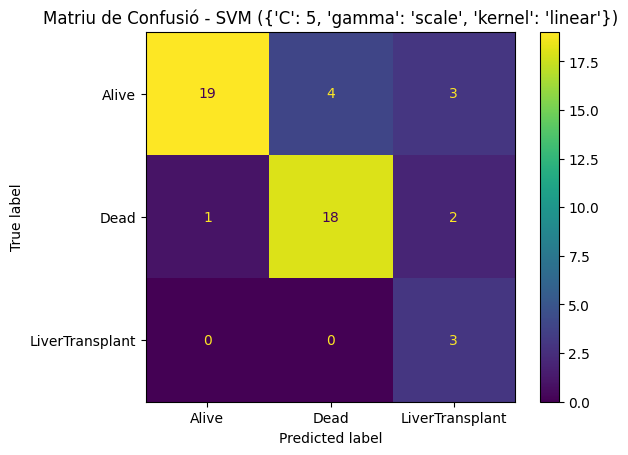
\includegraphics[width=0.85\linewidth]{img/svm-cm.png}
	\caption{Matriu de confusió de les prediccions del Support Vector Machine (amb paràmetres \textit{C = 5, gamma = `scale'} i \textit{kernel = `linear')} en el conjunt de test.}
	\label{fig:svm-cm}	
\end{figure}

En aquest model, la classe `Alive' s'ha predit correctament en una proporció de $\dfrac{19}{26} \approx 0,7308$ i en la classe `Dead' $\dfrac{18}{21} \approx 0,8571$. Aquests resultats són més semblants al KNN que no pas a l'Arbre de Decisió. no obstant la sorpresa, com ja s'ha dit, és que s'han predit correctament tots els valors de `LiverTransplant'.

Es pot dir que, en aquest model SVM, no hi ha pràcticament tendència a predir arbitràriament la classe majoritària perquè la majoria de falsos positius es troben quan es predeia `LiverTransplant' o `Dead' (classes minoritàries en comparació amb `Alive'), a més de que són les classes on hi ha més percentatge de prediccions correctes.

%--------------------------------------------------------------------------




\section{Selecció del model}

\subsection{Descripció del model triat}

\subsection{Anàlisi de les limitacions i capacitats del model}

\subsection{Resultats}



\section{Model Card per Support Vector Machine (SVM)}

\subsection{Informació General}
\begin{itemize}

\item \textbf{Nom del model}: SVM per a la predicció de l'estatus de pacients amb Cirrosi Hepàtica.
\item \textbf{Tipus de model}: Support Vector Machine (SVM).
\item \textbf{Font}: model general extret de la llibreria scikit-learn de Python.
\item \textbf{Desenvolupadors}: Cai Selvas Sala, estudiant del Grau en Intel·ligència Artificial de la Universitat Politècnica de Catalunya.
\item \textbf{Data de creació}: 28/12/2023
\item \textbf{Versió del model}: 1.0
\item \textbf{Descripció del Model}: El SVM és un model de classificació utilitzat per a predir l'estatus (`Alive', `Dead', `LiverTransplant') de pacients amb Cirrosi Hepàtica. Utilitza un kernel lineal per a separar les classes i ha estat entrenat amb un conjunt de dades que inclouen variables clíniques i demogràfiques.
\end{itemize}

\subsection{Hiperparàmetres}
Han estat determinats mitjançant una validació creuada amb \textit{K-Fold} ($k = 5$).
\begin{itemize}
	\item \textbf{Kernel}: s'ha utilitzat un kernel lineal.
	\item \textbf{C}: s'ha utilitzat el valor $C = 5$. No es recomana, però es pot modificar si es desitja.
	\begin{figure}[H]
	\centering
	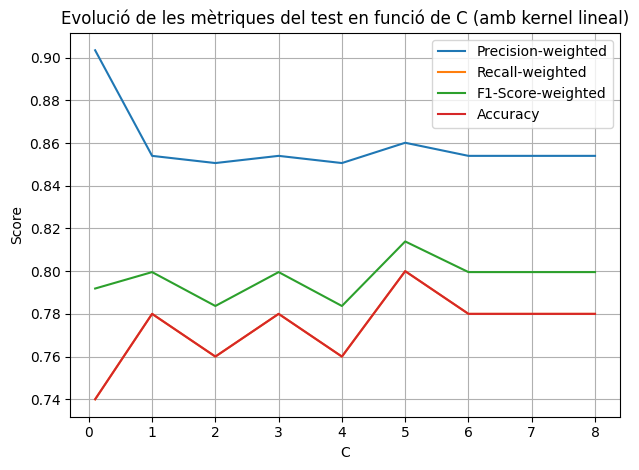
\includegraphics[width=0.5\linewidth]{img/c_evolution.png}
	\caption*{Evolucició de les mètriques en el test en funció del paràmetre C. \textit{Precision-weighted} i \textit{recall-weighted} es solapen en la gràfica, van junts.}
	\end{figure}
\end{itemize}

\subsection{Dades}
\begin{itemize}
\item \textbf{Font de les dades}: Estudi de Mayo Clinic sobre Cirrosis \cite{misc_cirrhosis_patient_survival_prediction_878}.
\item \textbf{Període de recopilació}: 1974 - 1948.
\item \textbf{Número de mostres inicials}: 418 pacients.
\item \textbf{Preprocessament}:
\begin{itemize}
	\item \textbf{Particionat en train i test}: 85\% train i 15\% test (amb el mètode \textit{stratify} per mantenir la distribució de classes).
	\item \textbf{Tractament d'outliers}: no s'han eliminat outliers.
	\item \textbf{Tractament de missings}: 
	\begin{itemize}
		\item \textbf{Eliminació de mostres}: no s'han considerat les mostres amb 9 valors faltants per garantir una millor qualitat de les dades.
		\item \textbf{Imputació de missings}: KNN Imputer ($k=15$) per variables numèriques. Random Forest Classifier (amb criteri `gini') per categoòriques.
	\end{itemize}
	\item \textbf{Codificació de variables}: variables categòriques codificades mitjançant \textit{Ordinal Encoding}.
	\item \textbf{Escalat de variables}: variables numèriques escalades a través de \textit{MinMax Scaler}.
	\item \textbf{Balanceig de classes}: mètode \textit{SMOTE} per a balancejar les classes de la variable objectiu (\textit{Status}). Amb això, el dataset d'entrenament consta de 441 mostres (pacients).
	\item \textbf{Característiques incloses}: Edat, Sexe, Resultats de laboratori (Presència o quantitat de Ascites, Hepatomegaly, Spiders, Edema, Cholesterol, Albumin, Copper, Alk\_Phos, SGOT, Tryglicerides, Platelets, Prothrombin), estat de la malaltia (Stage), dies del pacient en el tractament, administració del tractament o placebo, estat final del pacient.

\end{itemize}
\end{itemize}

\subsection{Validació}
\begin{itemize}
\item \textbf{Mida del conjunt de test}: 50 mostres (pacients). 
\item \textbf{Rendiment}:
\begin{itemize}
	\item \textbf{Rendiment mitjà en validació creuada}: F1-Score Weighted = 0,7463.
	\item \textbf{Rendiment en la validació (test)}:
	\begin{itemize}
		\item F1-Score Weighted = 0,8139.
		\item Accuracy = 0,8.
		\item Precision Weighted = 0.8601.
		\item Recall Weighted = 0.8.
	\end{itemize}
	\item Matriu de confusió:
	\begin{figure}[H]
	\centering
	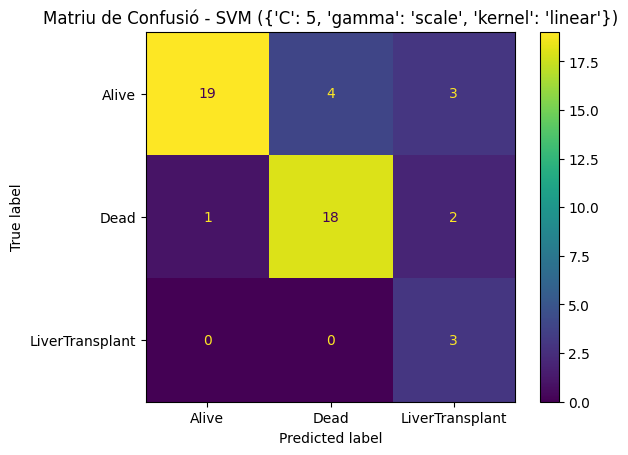
\includegraphics[width=0.6\linewidth]{img/svm-cm.png}
	\end{figure}
\end{itemize}
\end{itemize}

El rendiment pot variar segons la naturalesa del conjunt de dades de validació/test. Les prediccions de la classe `LiverTransplant' només han pogut ser provades amb les 3 mostres del conjunt de test, de manera que és difícil que es mantinguin els resultats que es mostren en la matriu de confusió. Generalment, el model tendeix a predir falsos positius en `LiverTransplant' i `Dead'.

\subsection{Advertències i Recomanacions}
Degut a desbalangeigs en atributs com ara \textit{Sex}, pot haver biaixos de sexe.

El model està dissenyat per a ser utilitzat com a eina de suport a la decisió clínica. En cap cas s'hauria d'utilitzar com a única font per a prendre decisions clíniques sensibles. Pot servir per fer una estimació de l'estat final d'un pacient amb Cirrosi per tal de prendre mesures sobre com guiar el seu tractament, però sempre sota la responsabilitat i aprovació d'un metge o professional especialitzat.

\subsection{Limitacions}
\begin{itemize}
\item Per funcionar correcatment amb dades externes, aquestes s'han de preprocessar de la mateixa manera en què el model ha estat entrenat.
\item EL model no és totalment precís, en certs casos pot predir una classe que no és correcta, tal i com es veu en la matriu de confusió.
\item El model pot tenir lleuger overfitting, de maner que els resultats siguin pitjors en un escenari real.
\end{itemize}

%-------------------------------------------------------------------------------------

\section{Bonus 1: Model EBM i comparació amb els models anteriors}
%Per aquells estudiants que assoleixin aquest punt, i vulguin fer un pas extra, poden entrenar un model de EBM i comparar amb els models anteriors. (1 Taula amb m`etriquees + 1 Figura amb les variables més importants en train/test)

\section{Bonus 2: Anàlisi no supervisat de les dades}
% Fer an`alisi no supervisat de les dades. Traient la variable ”Status”, podem identificar cl ́usters? A què corresponen? Ens poden servir per quelcom en la nostra tasca? I fora de la nostra tasca?

\section{Conclusions}
Durant la realització d'aquest projecte s'han apres (i sobretot consolidat) molts conceptes de Machine Learning (Aprenentatge Automàtic) i les seves aplicacions en el món real; en aquest cas, en l'àmbit de la salut.

Inicialment, ja s'ha vist que el dataset era complex i requeria un bon tractament per tal de els models fossin bons. Pel que fa al tractament que s'ha fet en aquest projecte, es podrien haver provat més mètodes d'imputació (o haver provat diferents paràmetres) per tal d'obtenir millors resultats. En un principi no semblava que la eliminació de files, outliers o els mètodes de imputació fossin tant determinants pels models, però s'ha acabat veient que canviaven molt el seu comportament.

El rendiment dels models generats semblava bo en un inici, però posteriorment s'ha vist (almenys pel model escollit), que els experiments s'haurien d'haver fet amb més llavors per tal de trobar models que realment generalitzessin millor i no destaquessin només en una llavor. No obstant, com ja s'ha dit al llarg del treball, l'objectiu d'aquesta pràctica ha esta provar diferents mètodes, models... i extreure'n un aprenentatge, de manera que es valora molt veure que certes coses podrien ser millorades, especialment si es tractés d'un model que realment s'hagués d'aplicar al món real. 

Addicionalment, ha quedat en evidència que els petits canvis en el dataset poden influir molt en els resultats dels models, i els propis resultats dels models poden ser molt enganyosos. En futurs projectes, s'haurà d'anar més en compte amb les mètriques i plantejar la creació de models des d'un altre punt de vista. És a dir, en aquest projecte s'han determinat molts paràmetres en funció de les puntuacions, i aquestes puntuacions han resultat ser enganyoses en certs casos, especialment quan es treballa amb una sola llavor. Seria una bona opció haver tingut més en compte altre mètriques més robustes i haver determinat els paràmetres també amb altres criteris.

Pel que fa a les prediccions i les conclusions de l'estudi, es pot dir que les diferències entre pacients amb classe `Alive' i `Dead' semblaven bastant clares. No obstant, els pacients amb `LiverTransplant' poden ser un problema pels models per la seva poca presència en el datset i perquè es desconeix els motius que porten a que un pacient pugui rebre un transplantament de fetge. Per altra banda, és curiós que les dades de l'estudi mostren que la variable \textit{Drug} (que indica si s'ha administrat el tractament o un placebo) és de les que menys influeix en la resposta, de manera que el tractament que es subministrava en aquest estudi no era útil. Totes aquestes coses remarquen la importància d'aquest estudi a nivell d'anàlisi, i no tant de rendiment dels models.

En referència al contingut que es requeria en aquesta pràctica, es considera que generalment s'ha assolit amb èxit. No obstant, com ja s'ha mencionat, hi ha certs aspectes que es podrien millorar (i que es milloraran en futurs projectes) per tal de proporcionar un anàlisi més complet i robust. Pel que fa als punts de bonus, no ha donat temps de poder realitzar-los tots, però s'ha inclòs una petita part del bonus 2, que si s'hagués disposat de més temps hagués pogut ser molt interessant.

Finalment, es pot concloure que l'aprenentatge adquirit en aquesta pràctica, tot i ser el primer contacte que es té amb l'aprenentatge automàtic, és immensament valuós per el grau que s'està cursant. Realment la intel·ligència artificial pot tenir grans usos en molts àmbits del món real, i en aquest projecte s'ha pogut apreciar la gran quantitat d'informació útil que es pot extreure d'una base de dades (tot i que aquesta tingui numerosos desperfectes) i aquest informació es pot utilitzar per generar models capaços de realitzar prediccions que poden ajudar a prendre moltes decisions en el món real.



\bibliographystyle{unsrt}
\bibliography{bibliography}


\end{document}

